% Created by tikzDevice version 0.10.1.2 on 2018-03-05 18:50:58
% !TEX encoding = UTF-8 Unicode
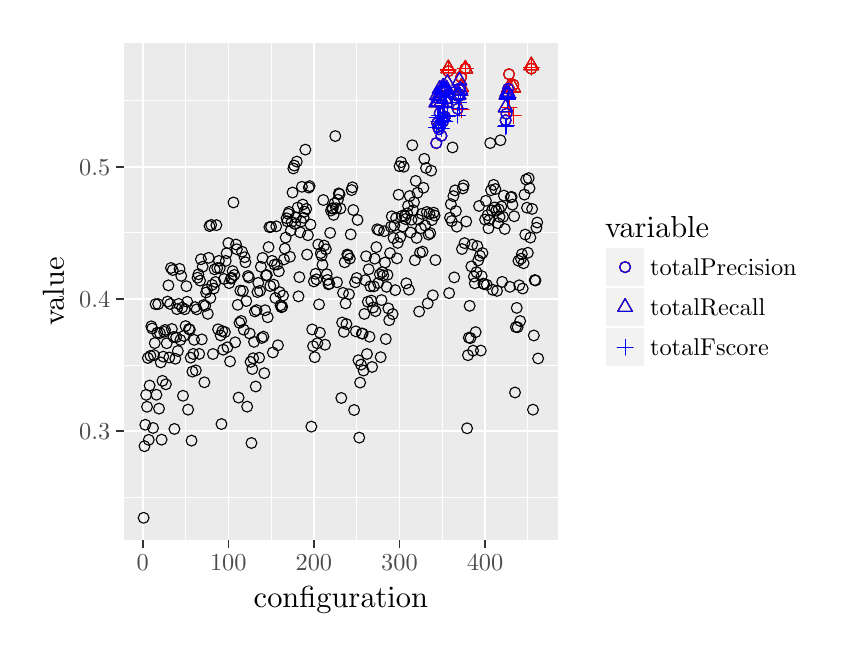
\begin{tikzpicture}[x=1pt,y=1pt]
\definecolor{fillColor}{RGB}{255,255,255}
\path[use as bounding box,fill=fillColor,fill opacity=0.00] (0,0) rectangle (289.08,216.81);
\begin{scope}
\path[clip] (  0.00,  0.00) rectangle (289.08,216.81);
\definecolor{drawColor}{RGB}{255,255,255}
\definecolor{fillColor}{RGB}{255,255,255}

\path[draw=drawColor,line width= 0.6pt,line join=round,line cap=round,fill=fillColor] (  0.00,  0.00) rectangle (289.08,216.81);
\end{scope}
\begin{scope}
\path[clip] ( 34.77, 31.53) rectangle (191.57,211.31);
\definecolor{fillColor}{gray}{0.92}

\path[fill=fillColor] ( 34.77, 31.53) rectangle (191.57,211.31);
\definecolor{drawColor}{RGB}{255,255,255}

\path[draw=drawColor,line width= 0.3pt,line join=round] ( 34.77, 47.11) --
	(191.57, 47.11);

\path[draw=drawColor,line width= 0.3pt,line join=round] ( 34.77, 94.90) --
	(191.57, 94.90);

\path[draw=drawColor,line width= 0.3pt,line join=round] ( 34.77,142.68) --
	(191.57,142.68);

\path[draw=drawColor,line width= 0.3pt,line join=round] ( 34.77,190.47) --
	(191.57,190.47);

\path[draw=drawColor,line width= 0.3pt,line join=round] ( 57.05, 31.53) --
	( 57.05,211.31);

\path[draw=drawColor,line width= 0.3pt,line join=round] ( 87.97, 31.53) --
	( 87.97,211.31);

\path[draw=drawColor,line width= 0.3pt,line join=round] (118.89, 31.53) --
	(118.89,211.31);

\path[draw=drawColor,line width= 0.3pt,line join=round] (149.81, 31.53) --
	(149.81,211.31);

\path[draw=drawColor,line width= 0.3pt,line join=round] (180.74, 31.53) --
	(180.74,211.31);

\path[draw=drawColor,line width= 0.6pt,line join=round] ( 34.77, 71.00) --
	(191.57, 71.00);

\path[draw=drawColor,line width= 0.6pt,line join=round] ( 34.77,118.79) --
	(191.57,118.79);

\path[draw=drawColor,line width= 0.6pt,line join=round] ( 34.77,166.58) --
	(191.57,166.58);

\path[draw=drawColor,line width= 0.6pt,line join=round] ( 41.59, 31.53) --
	( 41.59,211.31);

\path[draw=drawColor,line width= 0.6pt,line join=round] ( 72.51, 31.53) --
	( 72.51,211.31);

\path[draw=drawColor,line width= 0.6pt,line join=round] (103.43, 31.53) --
	(103.43,211.31);

\path[draw=drawColor,line width= 0.6pt,line join=round] (134.35, 31.53) --
	(134.35,211.31);

\path[draw=drawColor,line width= 0.6pt,line join=round] (165.27, 31.53) --
	(165.27,211.31);
\definecolor{drawColor}{RGB}{0,0,0}

\path[draw=drawColor,line width= 0.4pt,line join=round,line cap=round] ( 41.90, 39.70) circle (  1.96);

\path[draw=drawColor,line width= 0.4pt,line join=round,line cap=round] ( 42.20, 65.58) circle (  1.96);

\path[draw=drawColor,line width= 0.4pt,line join=round,line cap=round] ( 42.51, 73.32) circle (  1.96);

\path[draw=drawColor,line width= 0.4pt,line join=round,line cap=round] ( 42.82, 84.14) circle (  1.96);

\path[draw=drawColor,line width= 0.4pt,line join=round,line cap=round] ( 43.13, 79.82) circle (  1.96);

\path[draw=drawColor,line width= 0.4pt,line join=round,line cap=round] ( 43.44, 97.45) circle (  1.96);

\path[draw=drawColor,line width= 0.4pt,line join=round,line cap=round] ( 43.75, 67.87) circle (  1.96);

\path[draw=drawColor,line width= 0.4pt,line join=round,line cap=round] ( 44.06, 87.49) circle (  1.96);

\path[draw=drawColor,line width= 0.4pt,line join=round,line cap=round] ( 44.37, 98.22) circle (  1.96);

\path[draw=drawColor,line width= 0.4pt,line join=round,line cap=round] ( 44.68,108.90) circle (  1.96);

\path[draw=drawColor,line width= 0.4pt,line join=round,line cap=round] ( 44.99,108.11) circle (  1.96);

\path[draw=drawColor,line width= 0.4pt,line join=round,line cap=round] ( 45.30, 72.17) circle (  1.96);

\path[draw=drawColor,line width= 0.4pt,line join=round,line cap=round] ( 45.61, 98.48) circle (  1.96);

\path[draw=drawColor,line width= 0.4pt,line join=round,line cap=round] ( 45.92,102.83) circle (  1.96);

\path[draw=drawColor,line width= 0.4pt,line join=round,line cap=round] ( 46.22,116.90) circle (  1.96);

\path[draw=drawColor,line width= 0.4pt,line join=round,line cap=round] ( 46.53, 84.17) circle (  1.96);

\path[draw=drawColor,line width= 0.4pt,line join=round,line cap=round] ( 46.84,106.56) circle (  1.96);

\path[draw=drawColor,line width= 0.4pt,line join=round,line cap=round] ( 47.15,116.93) circle (  1.96);

\path[draw=drawColor,line width= 0.4pt,line join=round,line cap=round] ( 47.46, 79.15) circle (  1.96);

\path[draw=drawColor,line width= 0.4pt,line join=round,line cap=round] ( 47.77,106.44) circle (  1.96);

\path[draw=drawColor,line width= 0.4pt,line join=round,line cap=round] ( 48.08, 95.85) circle (  1.96);

\path[draw=drawColor,line width= 0.4pt,line join=round,line cap=round] ( 48.39, 67.94) circle (  1.96);

\path[draw=drawColor,line width= 0.4pt,line join=round,line cap=round] ( 48.70, 89.19) circle (  1.96);

\path[draw=drawColor,line width= 0.4pt,line join=round,line cap=round] ( 49.01, 97.93) circle (  1.96);

\path[draw=drawColor,line width= 0.4pt,line join=round,line cap=round] ( 49.32,106.91) circle (  1.96);

\path[draw=drawColor,line width= 0.4pt,line join=round,line cap=round] ( 49.63,107.58) circle (  1.96);

\path[draw=drawColor,line width= 0.4pt,line join=round,line cap=round] ( 49.94, 87.94) circle (  1.96);

\path[draw=drawColor,line width= 0.4pt,line join=round,line cap=round] ( 50.24,102.76) circle (  1.96);

\path[draw=drawColor,line width= 0.4pt,line join=round,line cap=round] ( 50.55,117.83) circle (  1.96);

\path[draw=drawColor,line width= 0.4pt,line join=round,line cap=round] ( 50.86,123.69) circle (  1.96);

\path[draw=drawColor,line width= 0.4pt,line join=round,line cap=round] ( 51.17, 97.62) circle (  1.96);

\path[draw=drawColor,line width= 0.4pt,line join=round,line cap=round] ( 51.48,116.97) circle (  1.96);

\path[draw=drawColor,line width= 0.4pt,line join=round,line cap=round] ( 51.79,129.97) circle (  1.96);

\path[draw=drawColor,line width= 0.4pt,line join=round,line cap=round] ( 52.10,107.92) circle (  1.96);

\path[draw=drawColor,line width= 0.4pt,line join=round,line cap=round] ( 52.41,129.23) circle (  1.96);

\path[draw=drawColor,line width= 0.4pt,line join=round,line cap=round] ( 52.72,105.05) circle (  1.96);

\path[draw=drawColor,line width= 0.4pt,line join=round,line cap=round] ( 53.03, 71.81) circle (  1.96);

\path[draw=drawColor,line width= 0.4pt,line join=round,line cap=round] ( 53.34, 97.17) circle (  1.96);

\path[draw=drawColor,line width= 0.4pt,line join=round,line cap=round] ( 53.65,104.93) circle (  1.96);

\path[draw=drawColor,line width= 0.4pt,line join=round,line cap=round] ( 53.95,115.11) circle (  1.96);

\path[draw=drawColor,line width= 0.4pt,line join=round,line cap=round] ( 54.26, 99.98) circle (  1.96);

\path[draw=drawColor,line width= 0.4pt,line join=round,line cap=round] ( 54.57,117.00) circle (  1.96);

\path[draw=drawColor,line width= 0.4pt,line join=round,line cap=round] ( 54.88,129.66) circle (  1.96);

\path[draw=drawColor,line width= 0.4pt,line join=round,line cap=round] ( 55.19,103.98) circle (  1.96);

\path[draw=drawColor,line width= 0.4pt,line join=round,line cap=round] ( 55.50,127.13) circle (  1.96);

\path[draw=drawColor,line width= 0.4pt,line join=round,line cap=round] ( 55.81,115.66) circle (  1.96);

\path[draw=drawColor,line width= 0.4pt,line join=round,line cap=round] ( 56.12, 83.79) circle (  1.96);

\path[draw=drawColor,line width= 0.4pt,line join=round,line cap=round] ( 56.43,105.43) circle (  1.96);

\path[draw=drawColor,line width= 0.4pt,line join=round,line cap=round] ( 56.74,115.06) circle (  1.96);

\path[draw=drawColor,line width= 0.4pt,line join=round,line cap=round] ( 57.05,108.97) circle (  1.96);

\path[draw=drawColor,line width= 0.4pt,line join=round,line cap=round] ( 57.36,123.38) circle (  1.96);

\path[draw=drawColor,line width= 0.4pt,line join=round,line cap=round] ( 57.67,117.76) circle (  1.96);

\path[draw=drawColor,line width= 0.4pt,line join=round,line cap=round] ( 57.97, 78.79) circle (  1.96);

\path[draw=drawColor,line width= 0.4pt,line join=round,line cap=round] ( 58.28,107.92) circle (  1.96);

\path[draw=drawColor,line width= 0.4pt,line join=round,line cap=round] ( 58.59,107.68) circle (  1.96);

\path[draw=drawColor,line width= 0.4pt,line join=round,line cap=round] ( 58.90, 97.57) circle (  1.96);

\path[draw=drawColor,line width= 0.4pt,line join=round,line cap=round] ( 59.21, 67.59) circle (  1.96);

\path[draw=drawColor,line width= 0.4pt,line join=round,line cap=round] ( 59.52, 92.53) circle (  1.96);

\path[draw=drawColor,line width= 0.4pt,line join=round,line cap=round] ( 59.83, 98.91) circle (  1.96);

\path[draw=drawColor,line width= 0.4pt,line join=round,line cap=round] ( 60.14,104.00) circle (  1.96);

\path[draw=drawColor,line width= 0.4pt,line join=round,line cap=round] ( 60.45,115.83) circle (  1.96);

\path[draw=drawColor,line width= 0.4pt,line join=round,line cap=round] ( 60.76, 92.98) circle (  1.96);

\path[draw=drawColor,line width= 0.4pt,line join=round,line cap=round] ( 61.07,115.01) circle (  1.96);

\path[draw=drawColor,line width= 0.4pt,line join=round,line cap=round] ( 61.38,126.46) circle (  1.96);

\path[draw=drawColor,line width= 0.4pt,line join=round,line cap=round] ( 61.69,127.70) circle (  1.96);

\path[draw=drawColor,line width= 0.4pt,line join=round,line cap=round] ( 61.99, 98.93) circle (  1.96);

\path[draw=drawColor,line width= 0.4pt,line join=round,line cap=round] ( 62.30,125.41) circle (  1.96);

\path[draw=drawColor,line width= 0.4pt,line join=round,line cap=round] ( 62.61,133.12) circle (  1.96);

\path[draw=drawColor,line width= 0.4pt,line join=round,line cap=round] ( 62.92,104.17) circle (  1.96);

\path[draw=drawColor,line width= 0.4pt,line join=round,line cap=round] ( 63.23,130.42) circle (  1.96);

\path[draw=drawColor,line width= 0.4pt,line join=round,line cap=round] ( 63.54,116.57) circle (  1.96);

\path[draw=drawColor,line width= 0.4pt,line join=round,line cap=round] ( 63.85, 88.66) circle (  1.96);

\path[draw=drawColor,line width= 0.4pt,line join=round,line cap=round] ( 64.16,116.28) circle (  1.96);

\path[draw=drawColor,line width= 0.4pt,line join=round,line cap=round] ( 64.47,121.11) circle (  1.96);

\path[draw=drawColor,line width= 0.4pt,line join=round,line cap=round] ( 64.78,122.16) circle (  1.96);

\path[draw=drawColor,line width= 0.4pt,line join=round,line cap=round] ( 65.09,113.41) circle (  1.96);

\path[draw=drawColor,line width= 0.4pt,line join=round,line cap=round] ( 65.40,133.63) circle (  1.96);

\path[draw=drawColor,line width= 0.4pt,line join=round,line cap=round] ( 65.71,145.12) circle (  1.96);

\path[draw=drawColor,line width= 0.4pt,line join=round,line cap=round] ( 66.01,119.10) circle (  1.96);

\path[draw=drawColor,line width= 0.4pt,line join=round,line cap=round] ( 66.32,145.53) circle (  1.96);

\path[draw=drawColor,line width= 0.4pt,line join=round,line cap=round] ( 66.63,123.85) circle (  1.96);

\path[draw=drawColor,line width= 0.4pt,line join=round,line cap=round] ( 66.94, 98.89) circle (  1.96);

\path[draw=drawColor,line width= 0.4pt,line join=round,line cap=round] ( 67.25,122.54) circle (  1.96);

\path[draw=drawColor,line width= 0.4pt,line join=round,line cap=round] ( 67.56,129.47) circle (  1.96);

\path[draw=drawColor,line width= 0.4pt,line join=round,line cap=round] ( 67.87,124.91) circle (  1.96);

\path[draw=drawColor,line width= 0.4pt,line join=round,line cap=round] ( 68.18,145.45) circle (  1.96);

\path[draw=drawColor,line width= 0.4pt,line join=round,line cap=round] ( 68.49,129.95) circle (  1.96);

\path[draw=drawColor,line width= 0.4pt,line join=round,line cap=round] ( 68.80,107.82) circle (  1.96);

\path[draw=drawColor,line width= 0.4pt,line join=round,line cap=round] ( 69.11,132.55) circle (  1.96);

\path[draw=drawColor,line width= 0.4pt,line join=round,line cap=round] ( 69.42,129.90) circle (  1.96);

\path[draw=drawColor,line width= 0.4pt,line join=round,line cap=round] ( 69.73,105.62) circle (  1.96);

\path[draw=drawColor,line width= 0.4pt,line join=round,line cap=round] ( 70.03, 73.58) circle (  1.96);

\path[draw=drawColor,line width= 0.4pt,line join=round,line cap=round] ( 70.34,107.18) circle (  1.96);

\path[draw=drawColor,line width= 0.4pt,line join=round,line cap=round] ( 70.65,100.44) circle (  1.96);

\path[draw=drawColor,line width= 0.4pt,line join=round,line cap=round] ( 70.96,126.00) circle (  1.96);

\path[draw=drawColor,line width= 0.4pt,line join=round,line cap=round] ( 71.27,106.79) circle (  1.96);

\path[draw=drawColor,line width= 0.4pt,line join=round,line cap=round] ( 71.58,132.53) circle (  1.96);

\path[draw=drawColor,line width= 0.4pt,line join=round,line cap=round] ( 71.89,135.30) circle (  1.96);

\path[draw=drawColor,line width= 0.4pt,line join=round,line cap=round] ( 72.20,101.32) circle (  1.96);

\path[draw=drawColor,line width= 0.4pt,line join=round,line cap=round] ( 72.51,138.98) circle (  1.96);

\path[draw=drawColor,line width= 0.4pt,line join=round,line cap=round] ( 72.82,124.50) circle (  1.96);

\path[draw=drawColor,line width= 0.4pt,line join=round,line cap=round] ( 73.13, 96.21) circle (  1.96);

\path[draw=drawColor,line width= 0.4pt,line join=round,line cap=round] ( 73.44,126.12) circle (  1.96);

\path[draw=drawColor,line width= 0.4pt,line join=round,line cap=round] ( 73.75,126.43) circle (  1.96);

\path[draw=drawColor,line width= 0.4pt,line join=round,line cap=round] ( 74.05,128.85) circle (  1.96);

\path[draw=drawColor,line width= 0.4pt,line join=round,line cap=round] ( 74.36,153.65) circle (  1.96);

\path[draw=drawColor,line width= 0.4pt,line join=round,line cap=round] ( 74.67,127.46) circle (  1.96);

\path[draw=drawColor,line width= 0.4pt,line join=round,line cap=round] ( 74.98,103.11) circle (  1.96);

\path[draw=drawColor,line width= 0.4pt,line join=round,line cap=round] ( 75.29,138.45) circle (  1.96);

\path[draw=drawColor,line width= 0.4pt,line join=round,line cap=round] ( 75.60,136.73) circle (  1.96);

\path[draw=drawColor,line width= 0.4pt,line join=round,line cap=round] ( 75.91,116.66) circle (  1.96);

\path[draw=drawColor,line width= 0.4pt,line join=round,line cap=round] ( 76.22, 83.14) circle (  1.96);

\path[draw=drawColor,line width= 0.4pt,line join=round,line cap=round] ( 76.53,110.16) circle (  1.96);

\path[draw=drawColor,line width= 0.4pt,line join=round,line cap=round] ( 76.84,121.80) circle (  1.96);

\path[draw=drawColor,line width= 0.4pt,line join=round,line cap=round] ( 77.15,110.83) circle (  1.96);

\path[draw=drawColor,line width= 0.4pt,line join=round,line cap=round] ( 77.46,135.85) circle (  1.96);

\path[draw=drawColor,line width= 0.4pt,line join=round,line cap=round] ( 77.77,121.66) circle (  1.96);

\path[draw=drawColor,line width= 0.4pt,line join=round,line cap=round] ( 78.07,107.68) circle (  1.96);

\path[draw=drawColor,line width= 0.4pt,line join=round,line cap=round] ( 78.38,133.87) circle (  1.96);

\path[draw=drawColor,line width= 0.4pt,line join=round,line cap=round] ( 78.69,132.03) circle (  1.96);

\path[draw=drawColor,line width= 0.4pt,line join=round,line cap=round] ( 79.00,118.02) circle (  1.96);

\path[draw=drawColor,line width= 0.4pt,line join=round,line cap=round] ( 79.31, 79.87) circle (  1.96);

\path[draw=drawColor,line width= 0.4pt,line join=round,line cap=round] ( 79.62,127.08) circle (  1.96);

\path[draw=drawColor,line width= 0.4pt,line join=round,line cap=round] ( 79.93,126.51) circle (  1.96);

\path[draw=drawColor,line width= 0.4pt,line join=round,line cap=round] ( 80.24,106.29) circle (  1.96);

\path[draw=drawColor,line width= 0.4pt,line join=round,line cap=round] ( 80.55, 96.04) circle (  1.96);

\path[draw=drawColor,line width= 0.4pt,line join=round,line cap=round] ( 80.86, 66.73) circle (  1.96);

\path[draw=drawColor,line width= 0.4pt,line join=round,line cap=round] ( 81.17, 93.46) circle (  1.96);

\path[draw=drawColor,line width= 0.4pt,line join=round,line cap=round] ( 81.48, 97.36) circle (  1.96);

\path[draw=drawColor,line width= 0.4pt,line join=round,line cap=round] ( 81.78,103.28) circle (  1.96);

\path[draw=drawColor,line width= 0.4pt,line join=round,line cap=round] ( 82.09,114.25) circle (  1.96);

\path[draw=drawColor,line width= 0.4pt,line join=round,line cap=round] ( 82.40, 87.15) circle (  1.96);

\path[draw=drawColor,line width= 0.4pt,line join=round,line cap=round] ( 82.71,114.75) circle (  1.96);

\path[draw=drawColor,line width= 0.4pt,line join=round,line cap=round] ( 83.02,121.27) circle (  1.96);

\path[draw=drawColor,line width= 0.4pt,line join=round,line cap=round] ( 83.33,124.59) circle (  1.96);

\path[draw=drawColor,line width= 0.4pt,line join=round,line cap=round] ( 83.64, 97.55) circle (  1.96);

\path[draw=drawColor,line width= 0.4pt,line join=round,line cap=round] ( 83.95,121.70) circle (  1.96);

\path[draw=drawColor,line width= 0.4pt,line join=round,line cap=round] ( 84.26,130.42) circle (  1.96);

\path[draw=drawColor,line width= 0.4pt,line join=round,line cap=round] ( 84.57,104.67) circle (  1.96);

\path[draw=drawColor,line width= 0.4pt,line join=round,line cap=round] ( 84.88,133.60) circle (  1.96);

\path[draw=drawColor,line width= 0.4pt,line join=round,line cap=round] ( 85.19,105.15) circle (  1.96);

\path[draw=drawColor,line width= 0.4pt,line join=round,line cap=round] ( 85.50, 91.96) circle (  1.96);

\path[draw=drawColor,line width= 0.4pt,line join=round,line cap=round] ( 85.80,114.70) circle (  1.96);

\path[draw=drawColor,line width= 0.4pt,line join=round,line cap=round] ( 86.11,127.25) circle (  1.96);

\path[draw=drawColor,line width= 0.4pt,line join=round,line cap=round] ( 86.42,127.39) circle (  1.96);

\path[draw=drawColor,line width= 0.4pt,line join=round,line cap=round] ( 86.73,112.17) circle (  1.96);

\path[draw=drawColor,line width= 0.4pt,line join=round,line cap=round] ( 87.04,137.52) circle (  1.96);

\path[draw=drawColor,line width= 0.4pt,line join=round,line cap=round] ( 87.35,144.74) circle (  1.96);

\path[draw=drawColor,line width= 0.4pt,line join=round,line cap=round] ( 87.66,123.45) circle (  1.96);

\path[draw=drawColor,line width= 0.4pt,line join=round,line cap=round] ( 87.97,144.83) circle (  1.96);

\path[draw=drawColor,line width= 0.4pt,line join=round,line cap=round] ( 88.28,132.55) circle (  1.96);

\path[draw=drawColor,line width= 0.4pt,line join=round,line cap=round] ( 88.59, 99.44) circle (  1.96);

\path[draw=drawColor,line width= 0.4pt,line join=round,line cap=round] ( 88.90,123.95) circle (  1.96);

\path[draw=drawColor,line width= 0.4pt,line join=round,line cap=round] ( 89.21,131.19) circle (  1.96);

\path[draw=drawColor,line width= 0.4pt,line join=round,line cap=round] ( 89.52,119.12) circle (  1.96);

\path[draw=drawColor,line width= 0.4pt,line join=round,line cap=round] ( 89.82,145.02) circle (  1.96);

\path[draw=drawColor,line width= 0.4pt,line join=round,line cap=round] ( 90.13,131.24) circle (  1.96);

\path[draw=drawColor,line width= 0.4pt,line join=round,line cap=round] ( 90.44,102.04) circle (  1.96);

\path[draw=drawColor,line width= 0.4pt,line join=round,line cap=round] ( 90.75,128.78) circle (  1.96);

\path[draw=drawColor,line width= 0.4pt,line join=round,line cap=round] ( 91.06,121.23) circle (  1.96);

\path[draw=drawColor,line width= 0.4pt,line join=round,line cap=round] ( 91.37,116.52) circle (  1.96);

\path[draw=drawColor,line width= 0.4pt,line join=round,line cap=round] ( 91.68,115.80) circle (  1.96);

\path[draw=drawColor,line width= 0.4pt,line join=round,line cap=round] ( 91.99,115.99) circle (  1.96);

\path[draw=drawColor,line width= 0.4pt,line join=round,line cap=round] ( 92.30,120.01) circle (  1.96);

\path[draw=drawColor,line width= 0.4pt,line join=round,line cap=round] ( 92.61,133.05) circle (  1.96);

\path[draw=drawColor,line width= 0.4pt,line join=round,line cap=round] ( 92.92,136.97) circle (  1.96);

\path[draw=drawColor,line width= 0.4pt,line join=round,line cap=round] ( 93.23,140.94) circle (  1.96);

\path[draw=drawColor,line width= 0.4pt,line join=round,line cap=round] ( 93.54,147.94) circle (  1.96);

\path[draw=drawColor,line width= 0.4pt,line join=round,line cap=round] ( 93.84,146.84) circle (  1.96);

\path[draw=drawColor,line width= 0.4pt,line join=round,line cap=round] ( 94.15,149.56) circle (  1.96);

\path[draw=drawColor,line width= 0.4pt,line join=round,line cap=round] ( 94.46,150.23) circle (  1.96);

\path[draw=drawColor,line width= 0.4pt,line join=round,line cap=round] ( 94.77,134.01) circle (  1.96);

\path[draw=drawColor,line width= 0.4pt,line join=round,line cap=round] ( 95.08,143.49) circle (  1.96);

\path[draw=drawColor,line width= 0.4pt,line join=round,line cap=round] ( 95.39,146.62) circle (  1.96);

\path[draw=drawColor,line width= 0.4pt,line join=round,line cap=round] ( 95.70,157.23) circle (  1.96);

\path[draw=drawColor,line width= 0.4pt,line join=round,line cap=round] ( 96.01,165.93) circle (  1.96);

\path[draw=drawColor,line width= 0.4pt,line join=round,line cap=round] ( 96.32,166.98) circle (  1.96);

\path[draw=drawColor,line width= 0.4pt,line join=round,line cap=round] ( 96.63,145.86) circle (  1.96);

\path[draw=drawColor,line width= 0.4pt,line join=round,line cap=round] ( 96.94,148.23) circle (  1.96);

\path[draw=drawColor,line width= 0.4pt,line join=round,line cap=round] ( 97.25,168.41) circle (  1.96);

\path[draw=drawColor,line width= 0.4pt,line join=round,line cap=round] ( 97.56,151.81) circle (  1.96);

\path[draw=drawColor,line width= 0.4pt,line join=round,line cap=round] ( 97.86,119.72) circle (  1.96);

\path[draw=drawColor,line width= 0.4pt,line join=round,line cap=round] ( 98.17,126.67) circle (  1.96);

\path[draw=drawColor,line width= 0.4pt,line join=round,line cap=round] ( 98.48,142.85) circle (  1.96);

\path[draw=drawColor,line width= 0.4pt,line join=round,line cap=round] ( 98.79,146.74) circle (  1.96);

\path[draw=drawColor,line width= 0.4pt,line join=round,line cap=round] ( 99.10,159.31) circle (  1.96);

\path[draw=drawColor,line width= 0.4pt,line join=round,line cap=round] ( 99.41,152.88) circle (  1.96);

\path[draw=drawColor,line width= 0.4pt,line join=round,line cap=round] ( 99.72,148.11) circle (  1.96);

\path[draw=drawColor,line width= 0.4pt,line join=round,line cap=round] (100.03,150.33) circle (  1.96);

\path[draw=drawColor,line width= 0.4pt,line join=round,line cap=round] (100.34,172.74) circle (  1.96);

\path[draw=drawColor,line width= 0.4pt,line join=round,line cap=round] (100.65,151.31) circle (  1.96);

\path[draw=drawColor,line width= 0.4pt,line join=round,line cap=round] (100.96,134.82) circle (  1.96);

\path[draw=drawColor,line width= 0.4pt,line join=round,line cap=round] (101.27,141.80) circle (  1.96);

\path[draw=drawColor,line width= 0.4pt,line join=round,line cap=round] (101.58,159.02) circle (  1.96);

\path[draw=drawColor,line width= 0.4pt,line join=round,line cap=round] (101.88,159.55) circle (  1.96);

\path[draw=drawColor,line width= 0.4pt,line join=round,line cap=round] (102.19,145.69) circle (  1.96);

\path[draw=drawColor,line width= 0.4pt,line join=round,line cap=round] (102.50, 72.65) circle (  1.96);

\path[draw=drawColor,line width= 0.4pt,line join=round,line cap=round] (102.81,107.77) circle (  1.96);

\path[draw=drawColor,line width= 0.4pt,line join=round,line cap=round] (103.12,101.71) circle (  1.96);

\path[draw=drawColor,line width= 0.4pt,line join=round,line cap=round] (103.43,125.10) circle (  1.96);

\path[draw=drawColor,line width= 0.4pt,line join=round,line cap=round] (103.74, 97.74) circle (  1.96);

\path[draw=drawColor,line width= 0.4pt,line join=round,line cap=round] (104.05,127.87) circle (  1.96);

\path[draw=drawColor,line width= 0.4pt,line join=round,line cap=round] (104.36,125.86) circle (  1.96);

\path[draw=drawColor,line width= 0.4pt,line join=round,line cap=round] (104.67,102.76) circle (  1.96);

\path[draw=drawColor,line width= 0.4pt,line join=round,line cap=round] (104.98,138.48) circle (  1.96);

\path[draw=drawColor,line width= 0.4pt,line join=round,line cap=round] (105.29,116.81) circle (  1.96);

\path[draw=drawColor,line width= 0.4pt,line join=round,line cap=round] (105.59,106.60) circle (  1.96);

\path[draw=drawColor,line width= 0.4pt,line join=round,line cap=round] (105.90,135.37) circle (  1.96);

\path[draw=drawColor,line width= 0.4pt,line join=round,line cap=round] (106.21,134.44) circle (  1.96);

\path[draw=drawColor,line width= 0.4pt,line join=round,line cap=round] (106.52,131.12) circle (  1.96);

\path[draw=drawColor,line width= 0.4pt,line join=round,line cap=round] (106.83,154.53) circle (  1.96);

\path[draw=drawColor,line width= 0.4pt,line join=round,line cap=round] (107.14,138.07) circle (  1.96);

\path[draw=drawColor,line width= 0.4pt,line join=round,line cap=round] (107.45,102.25) circle (  1.96);

\path[draw=drawColor,line width= 0.4pt,line join=round,line cap=round] (107.76,136.73) circle (  1.96);

\path[draw=drawColor,line width= 0.4pt,line join=round,line cap=round] (108.07,127.72) circle (  1.96);

\path[draw=drawColor,line width= 0.4pt,line join=round,line cap=round] (108.38,125.65) circle (  1.96);

\path[draw=drawColor,line width= 0.4pt,line join=round,line cap=round] (108.69,124.07) circle (  1.96);

\path[draw=drawColor,line width= 0.4pt,line join=round,line cap=round] (109.00,124.26) circle (  1.96);

\path[draw=drawColor,line width= 0.4pt,line join=round,line cap=round] (109.31,142.66) circle (  1.96);

\path[draw=drawColor,line width= 0.4pt,line join=round,line cap=round] (109.61,150.73) circle (  1.96);

\path[draw=drawColor,line width= 0.4pt,line join=round,line cap=round] (109.92,151.52) circle (  1.96);

\path[draw=drawColor,line width= 0.4pt,line join=round,line cap=round] (110.23,151.47) circle (  1.96);

\path[draw=drawColor,line width= 0.4pt,line join=round,line cap=round] (110.54,149.16) circle (  1.96);

\path[draw=drawColor,line width= 0.4pt,line join=round,line cap=round] (110.85,153.31) circle (  1.96);

\path[draw=drawColor,line width= 0.4pt,line join=round,line cap=round] (111.16,177.64) circle (  1.96);

\path[draw=drawColor,line width= 0.4pt,line join=round,line cap=round] (111.47,151.57) circle (  1.96);

\path[draw=drawColor,line width= 0.4pt,line join=round,line cap=round] (111.78,124.81) circle (  1.96);

\path[draw=drawColor,line width= 0.4pt,line join=round,line cap=round] (112.09,154.63) circle (  1.96);

\path[draw=drawColor,line width= 0.4pt,line join=round,line cap=round] (112.40,156.92) circle (  1.96);

\path[draw=drawColor,line width= 0.4pt,line join=round,line cap=round] (112.71,156.64) circle (  1.96);

\path[draw=drawColor,line width= 0.4pt,line join=round,line cap=round] (113.02,151.47) circle (  1.96);

\path[draw=drawColor,line width= 0.4pt,line join=round,line cap=round] (113.33, 83.00) circle (  1.96);

\path[draw=drawColor,line width= 0.4pt,line join=round,line cap=round] (113.63,110.26) circle (  1.96);

\path[draw=drawColor,line width= 0.4pt,line join=round,line cap=round] (113.94,120.99) circle (  1.96);

\path[draw=drawColor,line width= 0.4pt,line join=round,line cap=round] (114.25,106.89) circle (  1.96);

\path[draw=drawColor,line width= 0.4pt,line join=round,line cap=round] (114.56,132.03) circle (  1.96);

\path[draw=drawColor,line width= 0.4pt,line join=round,line cap=round] (114.87,117.16) circle (  1.96);

\path[draw=drawColor,line width= 0.4pt,line join=round,line cap=round] (115.18,109.71) circle (  1.96);

\path[draw=drawColor,line width= 0.4pt,line join=round,line cap=round] (115.49,134.84) circle (  1.96);

\path[draw=drawColor,line width= 0.4pt,line join=round,line cap=round] (115.80,134.49) circle (  1.96);

\path[draw=drawColor,line width= 0.4pt,line join=round,line cap=round] (116.11,120.49) circle (  1.96);

\path[draw=drawColor,line width= 0.4pt,line join=round,line cap=round] (116.42,133.36) circle (  1.96);

\path[draw=drawColor,line width= 0.4pt,line join=round,line cap=round] (116.73,142.11) circle (  1.96);

\path[draw=drawColor,line width= 0.4pt,line join=round,line cap=round] (117.04,158.12) circle (  1.96);

\path[draw=drawColor,line width= 0.4pt,line join=round,line cap=round] (117.35,159.12) circle (  1.96);

\path[draw=drawColor,line width= 0.4pt,line join=round,line cap=round] (117.65,150.93) circle (  1.96);

\path[draw=drawColor,line width= 0.4pt,line join=round,line cap=round] (117.96, 78.65) circle (  1.96);

\path[draw=drawColor,line width= 0.4pt,line join=round,line cap=round] (118.27,124.79) circle (  1.96);

\path[draw=drawColor,line width= 0.4pt,line join=round,line cap=round] (118.58,107.08) circle (  1.96);

\path[draw=drawColor,line width= 0.4pt,line join=round,line cap=round] (118.89,126.34) circle (  1.96);

\path[draw=drawColor,line width= 0.4pt,line join=round,line cap=round] (119.20,147.34) circle (  1.96);

\path[draw=drawColor,line width= 0.4pt,line join=round,line cap=round] (119.51, 96.64) circle (  1.96);

\path[draw=drawColor,line width= 0.4pt,line join=round,line cap=round] (119.82, 68.68) circle (  1.96);

\path[draw=drawColor,line width= 0.4pt,line join=round,line cap=round] (120.13, 88.56) circle (  1.96);

\path[draw=drawColor,line width= 0.4pt,line join=round,line cap=round] (120.44, 95.04) circle (  1.96);

\path[draw=drawColor,line width= 0.4pt,line join=round,line cap=round] (120.75,106.29) circle (  1.96);

\path[draw=drawColor,line width= 0.4pt,line join=round,line cap=round] (121.06,106.24) circle (  1.96);

\path[draw=drawColor,line width= 0.4pt,line join=round,line cap=round] (121.37, 92.91) circle (  1.96);

\path[draw=drawColor,line width= 0.4pt,line join=round,line cap=round] (121.67,113.37) circle (  1.96);

\path[draw=drawColor,line width= 0.4pt,line join=round,line cap=round] (121.98,125.57) circle (  1.96);

\path[draw=drawColor,line width= 0.4pt,line join=round,line cap=round] (122.29,134.20) circle (  1.96);

\path[draw=drawColor,line width= 0.4pt,line join=round,line cap=round] (122.60, 98.89) circle (  1.96);

\path[draw=drawColor,line width= 0.4pt,line join=round,line cap=round] (122.91,117.76) circle (  1.96);

\path[draw=drawColor,line width= 0.4pt,line join=round,line cap=round] (123.22,129.49) circle (  1.96);

\path[draw=drawColor,line width= 0.4pt,line join=round,line cap=round] (123.53,105.12) circle (  1.96);

\path[draw=drawColor,line width= 0.4pt,line join=round,line cap=round] (123.84,123.35) circle (  1.96);

\path[draw=drawColor,line width= 0.4pt,line join=round,line cap=round] (124.15,118.19) circle (  1.96);

\path[draw=drawColor,line width= 0.4pt,line join=round,line cap=round] (124.46, 94.20) circle (  1.96);

\path[draw=drawColor,line width= 0.4pt,line join=round,line cap=round] (124.77,115.66) circle (  1.96);

\path[draw=drawColor,line width= 0.4pt,line join=round,line cap=round] (125.08,123.33) circle (  1.96);

\path[draw=drawColor,line width= 0.4pt,line join=round,line cap=round] (125.39,133.34) circle (  1.96);

\path[draw=drawColor,line width= 0.4pt,line join=round,line cap=round] (125.69,114.39) circle (  1.96);

\path[draw=drawColor,line width= 0.4pt,line join=round,line cap=round] (126.00,137.50) circle (  1.96);

\path[draw=drawColor,line width= 0.4pt,line join=round,line cap=round] (126.31,143.97) circle (  1.96);

\path[draw=drawColor,line width= 0.4pt,line join=round,line cap=round] (126.62,124.52) circle (  1.96);

\path[draw=drawColor,line width= 0.4pt,line join=round,line cap=round] (126.93,143.64) circle (  1.96);

\path[draw=drawColor,line width= 0.4pt,line join=round,line cap=round] (127.24,127.68) circle (  1.96);

\path[draw=drawColor,line width= 0.4pt,line join=round,line cap=round] (127.55, 97.74) circle (  1.96);

\path[draw=drawColor,line width= 0.4pt,line join=round,line cap=round] (127.86,118.38) circle (  1.96);

\path[draw=drawColor,line width= 0.4pt,line join=round,line cap=round] (128.17,128.47) circle (  1.96);

\path[draw=drawColor,line width= 0.4pt,line join=round,line cap=round] (128.48,127.27) circle (  1.96);

\path[draw=drawColor,line width= 0.4pt,line join=round,line cap=round] (128.79,143.26) circle (  1.96);

\path[draw=drawColor,line width= 0.4pt,line join=round,line cap=round] (129.10,131.93) circle (  1.96);

\path[draw=drawColor,line width= 0.4pt,line join=round,line cap=round] (129.41,104.29) circle (  1.96);

\path[draw=drawColor,line width= 0.4pt,line join=round,line cap=round] (129.71,123.16) circle (  1.96);

\path[draw=drawColor,line width= 0.4pt,line join=round,line cap=round] (130.02,127.51) circle (  1.96);

\path[draw=drawColor,line width= 0.4pt,line join=round,line cap=round] (130.33,115.37) circle (  1.96);

\path[draw=drawColor,line width= 0.4pt,line join=round,line cap=round] (130.64,111.10) circle (  1.96);

\path[draw=drawColor,line width= 0.4pt,line join=round,line cap=round] (130.95,135.35) circle (  1.96);

\path[draw=drawColor,line width= 0.4pt,line join=round,line cap=round] (131.26,144.86) circle (  1.96);

\path[draw=drawColor,line width= 0.4pt,line join=round,line cap=round] (131.57,148.63) circle (  1.96);

\path[draw=drawColor,line width= 0.4pt,line join=round,line cap=round] (131.88,113.32) circle (  1.96);

\path[draw=drawColor,line width= 0.4pt,line join=round,line cap=round] (132.19,140.79) circle (  1.96);

\path[draw=drawColor,line width= 0.4pt,line join=round,line cap=round] (132.50,145.31) circle (  1.96);

\path[draw=drawColor,line width= 0.4pt,line join=round,line cap=round] (132.81,121.97) circle (  1.96);

\path[draw=drawColor,line width= 0.4pt,line join=round,line cap=round] (133.12,148.06) circle (  1.96);

\path[draw=drawColor,line width= 0.4pt,line join=round,line cap=round] (133.42,133.44) circle (  1.96);

\path[draw=drawColor,line width= 0.4pt,line join=round,line cap=round] (133.73,139.05) circle (  1.96);

\path[draw=drawColor,line width= 0.4pt,line join=round,line cap=round] (134.04,156.44) circle (  1.96);

\path[draw=drawColor,line width= 0.4pt,line join=round,line cap=round] (134.35,166.74) circle (  1.96);

\path[draw=drawColor,line width= 0.4pt,line join=round,line cap=round] (134.66,141.18) circle (  1.96);

\path[draw=drawColor,line width= 0.4pt,line join=round,line cap=round] (134.97,168.22) circle (  1.96);

\path[draw=drawColor,line width= 0.4pt,line join=round,line cap=round] (135.28,148.82) circle (  1.96);

\path[draw=drawColor,line width= 0.4pt,line join=round,line cap=round] (135.59,144.98) circle (  1.96);

\path[draw=drawColor,line width= 0.4pt,line join=round,line cap=round] (135.90,166.55) circle (  1.96);

\path[draw=drawColor,line width= 0.4pt,line join=round,line cap=round] (136.21,148.75) circle (  1.96);

\path[draw=drawColor,line width= 0.4pt,line join=round,line cap=round] (136.52,147.65) circle (  1.96);

\path[draw=drawColor,line width= 0.4pt,line join=round,line cap=round] (136.83,124.43) circle (  1.96);

\path[draw=drawColor,line width= 0.4pt,line join=round,line cap=round] (137.14,149.71) circle (  1.96);

\path[draw=drawColor,line width= 0.4pt,line join=round,line cap=round] (137.44,152.41) circle (  1.96);

\path[draw=drawColor,line width= 0.4pt,line join=round,line cap=round] (137.75,122.13) circle (  1.96);

\path[draw=drawColor,line width= 0.4pt,line join=round,line cap=round] (138.06,155.99) circle (  1.96);

\path[draw=drawColor,line width= 0.4pt,line join=round,line cap=round] (138.37,142.80) circle (  1.96);

\path[draw=drawColor,line width= 0.4pt,line join=round,line cap=round] (138.68,147.39) circle (  1.96);

\path[draw=drawColor,line width= 0.4pt,line join=round,line cap=round] (138.99,174.34) circle (  1.96);

\path[draw=drawColor,line width= 0.4pt,line join=round,line cap=round] (139.30,150.81) circle (  1.96);

\path[draw=drawColor,line width= 0.4pt,line join=round,line cap=round] (139.61,153.74) circle (  1.96);

\path[draw=drawColor,line width= 0.4pt,line join=round,line cap=round] (139.92,132.77) circle (  1.96);

\path[draw=drawColor,line width= 0.4pt,line join=round,line cap=round] (140.23,161.44) circle (  1.96);

\path[draw=drawColor,line width= 0.4pt,line join=round,line cap=round] (140.54,140.84) circle (  1.96);

\path[draw=drawColor,line width= 0.4pt,line join=round,line cap=round] (140.85,157.14) circle (  1.96);

\path[draw=drawColor,line width= 0.4pt,line join=round,line cap=round] (141.16,147.44) circle (  1.96);

\path[draw=drawColor,line width= 0.4pt,line join=round,line cap=round] (141.46,114.23) circle (  1.96);

\path[draw=drawColor,line width= 0.4pt,line join=round,line cap=round] (141.77,135.49) circle (  1.96);

\path[draw=drawColor,line width= 0.4pt,line join=round,line cap=round] (142.08,144.33) circle (  1.96);

\path[draw=drawColor,line width= 0.4pt,line join=round,line cap=round] (142.39,149.54) circle (  1.96);

\path[draw=drawColor,line width= 0.4pt,line join=round,line cap=round] (142.70,135.87) circle (  1.96);

\path[draw=drawColor,line width= 0.4pt,line join=round,line cap=round] (143.01,158.95) circle (  1.96);

\path[draw=drawColor,line width= 0.4pt,line join=round,line cap=round] (143.32,169.42) circle (  1.96);

\path[draw=drawColor,line width= 0.4pt,line join=round,line cap=round] (143.63,145.31) circle (  1.96);

\path[draw=drawColor,line width= 0.4pt,line join=round,line cap=round] (143.94,166.10) circle (  1.96);

\path[draw=drawColor,line width= 0.4pt,line join=round,line cap=round] (144.25,150.21) circle (  1.96);

\path[draw=drawColor,line width= 0.4pt,line join=round,line cap=round] (144.56,117.19) circle (  1.96);

\path[draw=drawColor,line width= 0.4pt,line join=round,line cap=round] (144.87,142.04) circle (  1.96);

\path[draw=drawColor,line width= 0.4pt,line join=round,line cap=round] (145.18,149.59) circle (  1.96);

\path[draw=drawColor,line width= 0.4pt,line join=round,line cap=round] (145.48,142.56) circle (  1.96);

\path[draw=drawColor,line width= 0.4pt,line join=round,line cap=round] (145.79,165.14) circle (  1.96);

\path[draw=drawColor,line width= 0.4pt,line join=round,line cap=round] (146.10,147.32) circle (  1.96);

\path[draw=drawColor,line width= 0.4pt,line join=round,line cap=round] (146.41,120.10) circle (  1.96);

\path[draw=drawColor,line width= 0.4pt,line join=round,line cap=round] (146.72,149.95) circle (  1.96);

\path[draw=drawColor,line width= 0.4pt,line join=round,line cap=round] (147.03,148.92) circle (  1.96);

\path[draw=drawColor,line width= 0.4pt,line join=round,line cap=round] (147.34,132.84) circle (  1.96);

\path[draw=drawColor,line width= 0.4pt,line join=round,line cap=round] (147.65,175.10) circle (  1.96);

\path[draw=drawColor,line width= 0.4pt,line join=round,line cap=round] (147.96,182.30) circle (  1.96);

\path[draw=drawColor,line width= 0.4pt,line join=round,line cap=round] (148.27,180.89) circle (  1.96);

\path[draw=drawColor,line width= 0.4pt,line join=round,line cap=round] (148.58,180.12) circle (  1.96);

\path[draw=drawColor,line width= 0.4pt,line join=round,line cap=round] (148.89,185.90) circle (  1.96);

\path[draw=drawColor,line width= 0.4pt,line join=round,line cap=round] (149.20,181.53) circle (  1.96);

\path[draw=drawColor,line width= 0.4pt,line join=round,line cap=round] (149.50,177.73) circle (  1.96);

\path[draw=drawColor,line width= 0.4pt,line join=round,line cap=round] (149.81,184.02) circle (  1.96);

\path[draw=drawColor,line width= 0.4pt,line join=round,line cap=round] (150.12,182.94) circle (  1.96);

\path[draw=drawColor,line width= 0.4pt,line join=round,line cap=round] (150.43,184.16) circle (  1.96);

\path[draw=drawColor,line width= 0.4pt,line join=round,line cap=round] (150.74,184.69) circle (  1.96);

\path[draw=drawColor,line width= 0.4pt,line join=round,line cap=round] (151.05,194.41) circle (  1.96);

\path[draw=drawColor,line width= 0.4pt,line join=round,line cap=round] (151.36,193.93) circle (  1.96);

\path[draw=drawColor,line width= 0.4pt,line join=round,line cap=round] (151.67,189.73) circle (  1.96);

\path[draw=drawColor,line width= 0.4pt,line join=round,line cap=round] (151.98,201.08) circle (  1.96);

\path[draw=drawColor,line width= 0.4pt,line join=round,line cap=round] (152.29,120.89) circle (  1.96);

\path[draw=drawColor,line width= 0.4pt,line join=round,line cap=round] (152.60,148.11) circle (  1.96);

\path[draw=drawColor,line width= 0.4pt,line join=round,line cap=round] (152.91,153.03) circle (  1.96);

\path[draw=drawColor,line width= 0.4pt,line join=round,line cap=round] (153.22,146.93) circle (  1.96);

\path[draw=drawColor,line width= 0.4pt,line join=round,line cap=round] (153.52,173.53) circle (  1.96);

\path[draw=drawColor,line width= 0.4pt,line join=round,line cap=round] (153.83,155.94) circle (  1.96);

\path[draw=drawColor,line width= 0.4pt,line join=round,line cap=round] (154.14,126.58) circle (  1.96);

\path[draw=drawColor,line width= 0.4pt,line join=round,line cap=round] (154.45,158.02) circle (  1.96);

\path[draw=drawColor,line width= 0.4pt,line join=round,line cap=round] (154.76,150.54) circle (  1.96);

\path[draw=drawColor,line width= 0.4pt,line join=round,line cap=round] (155.07,144.90) circle (  1.96);

\path[draw=drawColor,line width= 0.4pt,line join=round,line cap=round] (155.38,187.51) circle (  1.96);

\path[draw=drawColor,line width= 0.4pt,line join=round,line cap=round] (155.69,192.05) circle (  1.96);

\path[draw=drawColor,line width= 0.4pt,line join=round,line cap=round] (156.00,192.81) circle (  1.96);

\path[draw=drawColor,line width= 0.4pt,line join=round,line cap=round] (156.31,194.96) circle (  1.96);

\path[draw=drawColor,line width= 0.4pt,line join=round,line cap=round] (156.62,198.95) circle (  1.96);

\path[draw=drawColor,line width= 0.4pt,line join=round,line cap=round] (156.93,136.83) circle (  1.96);

\path[draw=drawColor,line width= 0.4pt,line join=round,line cap=round] (157.24,158.71) circle (  1.96);

\path[draw=drawColor,line width= 0.4pt,line join=round,line cap=round] (157.54,159.81) circle (  1.96);

\path[draw=drawColor,line width= 0.4pt,line join=round,line cap=round] (157.85,138.95) circle (  1.96);

\path[draw=drawColor,line width= 0.4pt,line join=round,line cap=round] (158.16,201.96) circle (  1.96);

\path[draw=drawColor,line width= 0.4pt,line join=round,line cap=round] (158.47,146.77) circle (  1.96);

\path[draw=drawColor,line width= 0.4pt,line join=round,line cap=round] (158.78, 72.05) circle (  1.96);

\path[draw=drawColor,line width= 0.4pt,line join=round,line cap=round] (159.09, 98.46) circle (  1.96);

\path[draw=drawColor,line width= 0.4pt,line join=round,line cap=round] (159.40,104.79) circle (  1.96);

\path[draw=drawColor,line width= 0.4pt,line join=round,line cap=round] (159.71,116.30) circle (  1.96);

\path[draw=drawColor,line width= 0.4pt,line join=round,line cap=round] (160.02,104.64) circle (  1.96);

\path[draw=drawColor,line width= 0.4pt,line join=round,line cap=round] (160.33,130.54) circle (  1.96);

\path[draw=drawColor,line width= 0.4pt,line join=round,line cap=round] (160.64,138.41) circle (  1.96);

\path[draw=drawColor,line width= 0.4pt,line join=round,line cap=round] (160.95,100.10) circle (  1.96);

\path[draw=drawColor,line width= 0.4pt,line join=round,line cap=round] (161.25,126.86) circle (  1.96);

\path[draw=drawColor,line width= 0.4pt,line join=round,line cap=round] (161.56,124.43) circle (  1.96);

\path[draw=drawColor,line width= 0.4pt,line join=round,line cap=round] (161.87,106.79) circle (  1.96);

\path[draw=drawColor,line width= 0.4pt,line join=round,line cap=round] (162.18,128.47) circle (  1.96);

\path[draw=drawColor,line width= 0.4pt,line join=round,line cap=round] (162.49,137.86) circle (  1.96);

\path[draw=drawColor,line width= 0.4pt,line join=round,line cap=round] (162.80,132.72) circle (  1.96);

\path[draw=drawColor,line width= 0.4pt,line join=round,line cap=round] (163.11,152.38) circle (  1.96);

\path[draw=drawColor,line width= 0.4pt,line join=round,line cap=round] (163.42,134.39) circle (  1.96);

\path[draw=drawColor,line width= 0.4pt,line join=round,line cap=round] (163.73,100.13) circle (  1.96);

\path[draw=drawColor,line width= 0.4pt,line join=round,line cap=round] (164.04,127.06) circle (  1.96);

\path[draw=drawColor,line width= 0.4pt,line join=round,line cap=round] (164.35,135.37) circle (  1.96);

\path[draw=drawColor,line width= 0.4pt,line join=round,line cap=round] (164.66,124.33) circle (  1.96);

\path[draw=drawColor,line width= 0.4pt,line join=round,line cap=round] (164.97,124.14) circle (  1.96);

\path[draw=drawColor,line width= 0.4pt,line join=round,line cap=round] (165.27,147.46) circle (  1.96);

\path[draw=drawColor,line width= 0.4pt,line join=round,line cap=round] (165.58,154.25) circle (  1.96);

\path[draw=drawColor,line width= 0.4pt,line join=round,line cap=round] (165.89,123.90) circle (  1.96);

\path[draw=drawColor,line width= 0.4pt,line join=round,line cap=round] (166.20,149.06) circle (  1.96);

\path[draw=drawColor,line width= 0.4pt,line join=round,line cap=round] (166.51,144.31) circle (  1.96);

\path[draw=drawColor,line width= 0.4pt,line join=round,line cap=round] (166.82,147.29) circle (  1.96);

\path[draw=drawColor,line width= 0.4pt,line join=round,line cap=round] (167.13,175.10) circle (  1.96);

\path[draw=drawColor,line width= 0.4pt,line join=round,line cap=round] (167.44,158.07) circle (  1.96);

\path[draw=drawColor,line width= 0.4pt,line join=round,line cap=round] (167.75,150.78) circle (  1.96);

\path[draw=drawColor,line width= 0.4pt,line join=round,line cap=round] (168.06,122.09) circle (  1.96);

\path[draw=drawColor,line width= 0.4pt,line join=round,line cap=round] (168.37,160.00) circle (  1.96);

\path[draw=drawColor,line width= 0.4pt,line join=round,line cap=round] (168.68,151.83) circle (  1.96);

\path[draw=drawColor,line width= 0.4pt,line join=round,line cap=round] (168.99,158.50) circle (  1.96);

\path[draw=drawColor,line width= 0.4pt,line join=round,line cap=round] (169.29,150.69) circle (  1.96);

\path[draw=drawColor,line width= 0.4pt,line join=round,line cap=round] (169.60,121.70) circle (  1.96);

\path[draw=drawColor,line width= 0.4pt,line join=round,line cap=round] (169.91,146.17) circle (  1.96);

\path[draw=drawColor,line width= 0.4pt,line join=round,line cap=round] (170.22,151.16) circle (  1.96);

\path[draw=drawColor,line width= 0.4pt,line join=round,line cap=round] (170.53,148.44) circle (  1.96);

\path[draw=drawColor,line width= 0.4pt,line join=round,line cap=round] (170.84,176.13) circle (  1.96);

\path[draw=drawColor,line width= 0.4pt,line join=round,line cap=round] (171.15,152.19) circle (  1.96);

\path[draw=drawColor,line width= 0.4pt,line join=round,line cap=round] (171.46,124.95) circle (  1.96);

\path[draw=drawColor,line width= 0.4pt,line join=round,line cap=round] (171.77,148.46) circle (  1.96);

\path[draw=drawColor,line width= 0.4pt,line join=round,line cap=round] (172.08,156.13) circle (  1.96);

\path[draw=drawColor,line width= 0.4pt,line join=round,line cap=round] (172.39,144.07) circle (  1.96);

\path[draw=drawColor,line width= 0.4pt,line join=round,line cap=round] (172.70,183.35) circle (  1.96);

\path[draw=drawColor,line width= 0.4pt,line join=round,line cap=round] (173.01,185.71) circle (  1.96);

\path[draw=drawColor,line width= 0.4pt,line join=round,line cap=round] (173.31,193.05) circle (  1.96);

\path[draw=drawColor,line width= 0.4pt,line join=round,line cap=round] (173.62,194.72) circle (  1.96);

\path[draw=drawColor,line width= 0.4pt,line join=round,line cap=round] (173.93,199.98) circle (  1.96);

\path[draw=drawColor,line width= 0.4pt,line join=round,line cap=round] (174.24,123.16) circle (  1.96);

\path[draw=drawColor,line width= 0.4pt,line join=round,line cap=round] (174.55,155.51) circle (  1.96);

\path[draw=drawColor,line width= 0.4pt,line join=round,line cap=round] (174.86,155.66) circle (  1.96);

\path[draw=drawColor,line width= 0.4pt,line join=round,line cap=round] (175.17,152.86) circle (  1.96);

\path[draw=drawColor,line width= 0.4pt,line join=round,line cap=round] (175.48,196.20) circle (  1.96);

\path[draw=drawColor,line width= 0.4pt,line join=round,line cap=round] (175.79,148.66) circle (  1.96);

\path[draw=drawColor,line width= 0.4pt,line join=round,line cap=round] (176.10, 84.98) circle (  1.96);

\path[draw=drawColor,line width= 0.4pt,line join=round,line cap=round] (176.41,108.63) circle (  1.96);

\path[draw=drawColor,line width= 0.4pt,line join=round,line cap=round] (176.72,115.56) circle (  1.96);

\path[draw=drawColor,line width= 0.4pt,line join=round,line cap=round] (177.03,108.56) circle (  1.96);

\path[draw=drawColor,line width= 0.4pt,line join=round,line cap=round] (177.33,132.58) circle (  1.96);

\path[draw=drawColor,line width= 0.4pt,line join=round,line cap=round] (177.64,123.71) circle (  1.96);

\path[draw=drawColor,line width= 0.4pt,line join=round,line cap=round] (177.95,110.81) circle (  1.96);

\path[draw=drawColor,line width= 0.4pt,line join=round,line cap=round] (178.26,133.32) circle (  1.96);

\path[draw=drawColor,line width= 0.4pt,line join=round,line cap=round] (178.57,134.96) circle (  1.96);

\path[draw=drawColor,line width= 0.4pt,line join=round,line cap=round] (178.88,122.54) circle (  1.96);

\path[draw=drawColor,line width= 0.4pt,line join=round,line cap=round] (179.19,131.69) circle (  1.96);

\path[draw=drawColor,line width= 0.4pt,line join=round,line cap=round] (179.50,156.49) circle (  1.96);

\path[draw=drawColor,line width= 0.4pt,line join=round,line cap=round] (179.81,142.04) circle (  1.96);

\path[draw=drawColor,line width= 0.4pt,line join=round,line cap=round] (180.12,161.94) circle (  1.96);

\path[draw=drawColor,line width= 0.4pt,line join=round,line cap=round] (180.43,151.76) circle (  1.96);

\path[draw=drawColor,line width= 0.4pt,line join=round,line cap=round] (180.74,135.47) circle (  1.96);

\path[draw=drawColor,line width= 0.4pt,line join=round,line cap=round] (181.05,162.44) circle (  1.96);

\path[draw=drawColor,line width= 0.4pt,line join=round,line cap=round] (181.35,158.81) circle (  1.96);

\path[draw=drawColor,line width= 0.4pt,line join=round,line cap=round] (181.66,140.96) circle (  1.96);

\path[draw=drawColor,line width= 0.4pt,line join=round,line cap=round] (181.97,202.03) circle (  1.96);

\path[draw=drawColor,line width= 0.4pt,line join=round,line cap=round] (182.28,151.31) circle (  1.96);

\path[draw=drawColor,line width= 0.4pt,line join=round,line cap=round] (182.59, 78.77) circle (  1.96);

\path[draw=drawColor,line width= 0.4pt,line join=round,line cap=round] (182.90,105.58) circle (  1.96);

\path[draw=drawColor,line width= 0.4pt,line join=round,line cap=round] (183.21,125.60) circle (  1.96);

\path[draw=drawColor,line width= 0.4pt,line join=round,line cap=round] (183.52,125.45) circle (  1.96);

\path[draw=drawColor,line width= 0.4pt,line join=round,line cap=round] (183.83,144.52) circle (  1.96);

\path[draw=drawColor,line width= 0.4pt,line join=round,line cap=round] (184.14,146.41) circle (  1.96);

\path[draw=drawColor,line width= 0.4pt,line join=round,line cap=round] (184.45, 97.28) circle (  1.96);

\path[draw=drawColor,line width= 0.4pt,line join=round,line cap=round] (147.65,192.80) --
	(150.29,188.22) --
	(145.01,188.22) --
	(147.65,192.80);

\path[draw=drawColor,line width= 0.4pt,line join=round,line cap=round] (147.96,195.45) --
	(150.60,190.87) --
	(145.32,190.87) --
	(147.96,195.45);

\path[draw=drawColor,line width= 0.4pt,line join=round,line cap=round] (148.27,193.08) --
	(150.91,188.50) --
	(145.63,188.50) --
	(148.27,193.08);

\path[draw=drawColor,line width= 0.4pt,line join=round,line cap=round] (148.58,195.07) --
	(151.22,190.49) --
	(145.93,190.49) --
	(148.58,195.07);

\path[draw=drawColor,line width= 0.4pt,line join=round,line cap=round] (148.89,197.68) --
	(151.53,193.10) --
	(146.24,193.10) --
	(148.89,197.68);

\path[draw=drawColor,line width= 0.4pt,line join=round,line cap=round] (149.20,194.30) --
	(151.84,189.72) --
	(146.55,189.72) --
	(149.20,194.30);

\path[draw=drawColor,line width= 0.4pt,line join=round,line cap=round] (149.50,192.94) --
	(152.15,188.37) --
	(146.86,188.37) --
	(149.50,192.94);

\path[draw=drawColor,line width= 0.4pt,line join=round,line cap=round] (149.81,197.49) --
	(152.46,192.91) --
	(147.17,192.91) --
	(149.81,197.49);

\path[draw=drawColor,line width= 0.4pt,line join=round,line cap=round] (150.12,198.50) --
	(152.77,193.92) --
	(147.48,193.92) --
	(150.12,198.50);

\path[draw=drawColor,line width= 0.4pt,line join=round,line cap=round] (150.43,197.40) --
	(153.07,192.82) --
	(147.79,192.82) --
	(150.43,197.40);

\path[draw=drawColor,line width= 0.4pt,line join=round,line cap=round] (150.74,194.07) --
	(153.38,189.49) --
	(148.10,189.49) --
	(150.74,194.07);

\path[draw=drawColor,line width= 0.4pt,line join=round,line cap=round] (151.05,197.26) --
	(153.69,192.68) --
	(148.41,192.68) --
	(151.05,197.26);

\path[draw=drawColor,line width= 0.4pt,line join=round,line cap=round] (151.36,197.77) --
	(154.00,193.19) --
	(148.72,193.19) --
	(151.36,197.77);

\path[draw=drawColor,line width= 0.4pt,line join=round,line cap=round] (151.67,199.82) --
	(154.31,195.25) --
	(149.03,195.25) --
	(151.67,199.82);

\path[draw=drawColor,line width= 0.4pt,line join=round,line cap=round] (151.98,205.07) --
	(154.62,200.50) --
	(149.34,200.50) --
	(151.98,205.07);

\path[draw=drawColor,line width= 0.4pt,line join=round,line cap=round] (155.38,195.39) --
	(158.02,190.81) --
	(152.74,190.81) --
	(155.38,195.39);

\path[draw=drawColor,line width= 0.4pt,line join=round,line cap=round] (155.69,195.63) --
	(158.33,191.05) --
	(153.05,191.05) --
	(155.69,195.63);

\path[draw=drawColor,line width= 0.4pt,line join=round,line cap=round] (156.00,200.67) --
	(158.64,196.09) --
	(153.36,196.09) --
	(156.00,200.67);

\path[draw=drawColor,line width= 0.4pt,line join=round,line cap=round] (156.31,197.40) --
	(158.95,192.82) --
	(153.66,192.82) --
	(156.31,197.40);

\path[draw=drawColor,line width= 0.4pt,line join=round,line cap=round] (156.62,198.34) --
	(159.26,193.76) --
	(153.97,193.76) --
	(156.62,198.34);

\path[draw=drawColor,line width= 0.4pt,line join=round,line cap=round] (158.16,204.97) --
	(160.81,200.39) --
	(155.52,200.39) --
	(158.16,204.97);

\path[draw=drawColor,line width= 0.4pt,line join=round,line cap=round] (172.70,190.99) --
	(175.34,186.41) --
	(170.05,186.41) --
	(172.70,190.99);

\path[draw=drawColor,line width= 0.4pt,line join=round,line cap=round] (173.01,195.56) --
	(175.65,190.98) --
	(170.36,190.98) --
	(173.01,195.56);

\path[draw=drawColor,line width= 0.4pt,line join=round,line cap=round] (173.31,196.60) --
	(175.96,192.03) --
	(170.67,192.03) --
	(173.31,196.60);

\path[draw=drawColor,line width= 0.4pt,line join=round,line cap=round] (173.62,195.73) --
	(176.27,191.15) --
	(170.98,191.15) --
	(173.62,195.73);

\path[draw=drawColor,line width= 0.4pt,line join=round,line cap=round] (173.93,198.27) --
	(176.58,193.69) --
	(171.29,193.69) --
	(173.93,198.27);

\path[draw=drawColor,line width= 0.4pt,line join=round,line cap=round] (175.48,198.15) --
	(178.12,193.58) --
	(172.84,193.58) --
	(175.48,198.15);

\path[draw=drawColor,line width= 0.4pt,line join=round,line cap=round] (181.97,206.19) --
	(184.62,201.61) --
	(179.33,201.61) --
	(181.97,206.19);

\path[draw=drawColor,line width= 0.4pt,line join=round,line cap=round] (144.87,180.73) -- (150.42,180.73);

\path[draw=drawColor,line width= 0.4pt,line join=round,line cap=round] (147.65,177.95) -- (147.65,183.50);

\path[draw=drawColor,line width= 0.4pt,line join=round,line cap=round] (145.18,184.46) -- (150.73,184.46);

\path[draw=drawColor,line width= 0.4pt,line join=round,line cap=round] (147.96,181.69) -- (147.96,187.24);

\path[draw=drawColor,line width= 0.4pt,line join=round,line cap=round] (145.49,184.47) -- (151.04,184.47);

\path[draw=drawColor,line width= 0.4pt,line join=round,line cap=round] (148.27,181.69) -- (148.27,187.24);

\path[draw=drawColor,line width= 0.4pt,line join=round,line cap=round] (145.80,182.80) -- (151.35,182.80);

\path[draw=drawColor,line width= 0.4pt,line join=round,line cap=round] (148.58,180.02) -- (148.58,185.57);

\path[draw=drawColor,line width= 0.4pt,line join=round,line cap=round] (146.11,185.21) -- (151.66,185.21);

\path[draw=drawColor,line width= 0.4pt,line join=round,line cap=round] (148.89,182.44) -- (148.89,187.99);

\path[draw=drawColor,line width= 0.4pt,line join=round,line cap=round] (146.42,185.19) -- (151.97,185.19);

\path[draw=drawColor,line width= 0.4pt,line join=round,line cap=round] (149.20,182.42) -- (149.20,187.97);

\path[draw=drawColor,line width= 0.4pt,line join=round,line cap=round] (146.73,180.45) -- (152.28,180.45);

\path[draw=drawColor,line width= 0.4pt,line join=round,line cap=round] (149.50,177.67) -- (149.50,183.22);

\path[draw=drawColor,line width= 0.4pt,line join=round,line cap=round] (147.04,183.97) -- (152.59,183.97);

\path[draw=drawColor,line width= 0.4pt,line join=round,line cap=round] (149.81,181.19) -- (149.81,186.74);

\path[draw=drawColor,line width= 0.4pt,line join=round,line cap=round] (147.35,183.09) -- (152.90,183.09);

\path[draw=drawColor,line width= 0.4pt,line join=round,line cap=round] (150.12,180.32) -- (150.12,185.87);

\path[draw=drawColor,line width= 0.4pt,line join=round,line cap=round] (147.66,188.12) -- (153.21,188.12);

\path[draw=drawColor,line width= 0.4pt,line join=round,line cap=round] (150.43,185.34) -- (150.43,190.89);

\path[draw=drawColor,line width= 0.4pt,line join=round,line cap=round] (147.97,182.99) -- (153.52,182.99);

\path[draw=drawColor,line width= 0.4pt,line join=round,line cap=round] (150.74,180.22) -- (150.74,185.77);

\path[draw=drawColor,line width= 0.4pt,line join=round,line cap=round] (148.28,191.73) -- (153.83,191.73);

\path[draw=drawColor,line width= 0.4pt,line join=round,line cap=round] (151.05,188.95) -- (151.05,194.50);

\path[draw=drawColor,line width= 0.4pt,line join=round,line cap=round] (148.58,191.87) -- (154.13,191.87);

\path[draw=drawColor,line width= 0.4pt,line join=round,line cap=round] (151.36,189.10) -- (151.36,194.65);

\path[draw=drawColor,line width= 0.4pt,line join=round,line cap=round] (148.89,184.73) -- (154.44,184.73);

\path[draw=drawColor,line width= 0.4pt,line join=round,line cap=round] (151.67,181.96) -- (151.67,187.51);

\path[draw=drawColor,line width= 0.4pt,line join=round,line cap=round] (149.20,201.52) -- (154.75,201.52);

\path[draw=drawColor,line width= 0.4pt,line join=round,line cap=round] (151.98,198.75) -- (151.98,204.30);

\path[draw=drawColor,line width= 0.4pt,line join=round,line cap=round] (152.60,185.20) -- (158.15,185.20);

\path[draw=drawColor,line width= 0.4pt,line join=round,line cap=round] (155.38,182.42) -- (155.38,187.97);

\path[draw=drawColor,line width= 0.4pt,line join=round,line cap=round] (152.91,189.81) -- (158.46,189.81);

\path[draw=drawColor,line width= 0.4pt,line join=round,line cap=round] (155.69,187.03) -- (155.69,192.58);

\path[draw=drawColor,line width= 0.4pt,line join=round,line cap=round] (153.22,187.73) -- (158.77,187.73);

\path[draw=drawColor,line width= 0.4pt,line join=round,line cap=round] (156.00,184.95) -- (156.00,190.50);

\path[draw=drawColor,line width= 0.4pt,line join=round,line cap=round] (153.53,192.32) -- (159.08,192.32);

\path[draw=drawColor,line width= 0.4pt,line join=round,line cap=round] (156.31,189.55) -- (156.31,195.10);

\path[draw=drawColor,line width= 0.4pt,line join=round,line cap=round] (153.84,187.09) -- (159.39,187.09);

\path[draw=drawColor,line width= 0.4pt,line join=round,line cap=round] (156.62,184.32) -- (156.62,189.87);

\path[draw=drawColor,line width= 0.4pt,line join=round,line cap=round] (155.39,201.91) -- (160.94,201.91);

\path[draw=drawColor,line width= 0.4pt,line join=round,line cap=round] (158.16,199.14) -- (158.16,204.68);

\path[draw=drawColor,line width= 0.4pt,line join=round,line cap=round] (169.92,180.94) -- (175.47,180.94);

\path[draw=drawColor,line width= 0.4pt,line join=round,line cap=round] (172.70,178.16) -- (172.70,183.71);

\path[draw=drawColor,line width= 0.4pt,line join=round,line cap=round] (170.23,181.33) -- (175.78,181.33);

\path[draw=drawColor,line width= 0.4pt,line join=round,line cap=round] (173.01,178.55) -- (173.01,184.10);

\path[draw=drawColor,line width= 0.4pt,line join=round,line cap=round] (170.54,190.75) -- (176.09,190.75);

\path[draw=drawColor,line width= 0.4pt,line join=round,line cap=round] (173.31,187.98) -- (173.31,193.53);

\path[draw=drawColor,line width= 0.4pt,line join=round,line cap=round] (170.85,191.42) -- (176.40,191.42);

\path[draw=drawColor,line width= 0.4pt,line join=round,line cap=round] (173.62,188.65) -- (173.62,194.20);

\path[draw=drawColor,line width= 0.4pt,line join=round,line cap=round] (171.16,187.91) -- (176.71,187.91);

\path[draw=drawColor,line width= 0.4pt,line join=round,line cap=round] (173.93,185.13) -- (173.93,190.68);

\path[draw=drawColor,line width= 0.4pt,line join=round,line cap=round] (172.70,185.13) -- (178.25,185.13);

\path[draw=drawColor,line width= 0.4pt,line join=round,line cap=round] (175.48,182.36) -- (175.48,187.91);

\path[draw=drawColor,line width= 0.4pt,line join=round,line cap=round] (179.20,202.56) -- (184.75,202.56);

\path[draw=drawColor,line width= 0.4pt,line join=round,line cap=round] (181.97,199.78) -- (181.97,205.33);
\definecolor{drawColor}{RGB}{255,0,0}

\path[draw=drawColor,line width= 0.4pt,line join=round,line cap=round] (147.65,175.10) circle (  1.96);

\path[draw=drawColor,line width= 0.4pt,line join=round,line cap=round] (147.96,182.30) circle (  1.96);

\path[draw=drawColor,line width= 0.4pt,line join=round,line cap=round] (148.27,180.89) circle (  1.96);

\path[draw=drawColor,line width= 0.4pt,line join=round,line cap=round] (148.58,180.12) circle (  1.96);

\path[draw=drawColor,line width= 0.4pt,line join=round,line cap=round] (148.89,185.90) circle (  1.96);

\path[draw=drawColor,line width= 0.4pt,line join=round,line cap=round] (149.20,181.53) circle (  1.96);

\path[draw=drawColor,line width= 0.4pt,line join=round,line cap=round] (149.50,177.73) circle (  1.96);

\path[draw=drawColor,line width= 0.4pt,line join=round,line cap=round] (149.81,184.02) circle (  1.96);

\path[draw=drawColor,line width= 0.4pt,line join=round,line cap=round] (150.12,182.94) circle (  1.96);

\path[draw=drawColor,line width= 0.4pt,line join=round,line cap=round] (150.43,184.16) circle (  1.96);

\path[draw=drawColor,line width= 0.4pt,line join=round,line cap=round] (150.74,184.69) circle (  1.96);

\path[draw=drawColor,line width= 0.4pt,line join=round,line cap=round] (151.05,194.41) circle (  1.96);

\path[draw=drawColor,line width= 0.4pt,line join=round,line cap=round] (151.36,193.93) circle (  1.96);

\path[draw=drawColor,line width= 0.4pt,line join=round,line cap=round] (151.67,189.73) circle (  1.96);

\path[draw=drawColor,line width= 0.4pt,line join=round,line cap=round] (151.98,201.08) circle (  1.96);

\path[draw=drawColor,line width= 0.4pt,line join=round,line cap=round] (155.38,187.51) circle (  1.96);

\path[draw=drawColor,line width= 0.4pt,line join=round,line cap=round] (155.69,192.05) circle (  1.96);

\path[draw=drawColor,line width= 0.4pt,line join=round,line cap=round] (156.00,192.81) circle (  1.96);

\path[draw=drawColor,line width= 0.4pt,line join=round,line cap=round] (156.31,194.96) circle (  1.96);

\path[draw=drawColor,line width= 0.4pt,line join=round,line cap=round] (156.62,198.95) circle (  1.96);

\path[draw=drawColor,line width= 0.4pt,line join=round,line cap=round] (158.16,201.96) circle (  1.96);

\path[draw=drawColor,line width= 0.4pt,line join=round,line cap=round] (172.70,183.35) circle (  1.96);

\path[draw=drawColor,line width= 0.4pt,line join=round,line cap=round] (173.01,185.71) circle (  1.96);

\path[draw=drawColor,line width= 0.4pt,line join=round,line cap=round] (173.31,193.05) circle (  1.96);

\path[draw=drawColor,line width= 0.4pt,line join=round,line cap=round] (173.62,194.72) circle (  1.96);

\path[draw=drawColor,line width= 0.4pt,line join=round,line cap=round] (173.93,199.98) circle (  1.96);

\path[draw=drawColor,line width= 0.4pt,line join=round,line cap=round] (175.48,196.20) circle (  1.96);

\path[draw=drawColor,line width= 0.4pt,line join=round,line cap=round] (181.97,202.03) circle (  1.96);

\path[draw=drawColor,line width= 0.4pt,line join=round,line cap=round] (147.65,192.80) --
	(150.29,188.22) --
	(145.01,188.22) --
	(147.65,192.80);

\path[draw=drawColor,line width= 0.4pt,line join=round,line cap=round] (147.96,195.45) --
	(150.60,190.87) --
	(145.32,190.87) --
	(147.96,195.45);

\path[draw=drawColor,line width= 0.4pt,line join=round,line cap=round] (148.27,193.08) --
	(150.91,188.50) --
	(145.63,188.50) --
	(148.27,193.08);

\path[draw=drawColor,line width= 0.4pt,line join=round,line cap=round] (148.58,195.07) --
	(151.22,190.49) --
	(145.93,190.49) --
	(148.58,195.07);

\path[draw=drawColor,line width= 0.4pt,line join=round,line cap=round] (148.89,197.68) --
	(151.53,193.10) --
	(146.24,193.10) --
	(148.89,197.68);

\path[draw=drawColor,line width= 0.4pt,line join=round,line cap=round] (149.20,194.30) --
	(151.84,189.72) --
	(146.55,189.72) --
	(149.20,194.30);

\path[draw=drawColor,line width= 0.4pt,line join=round,line cap=round] (149.50,192.94) --
	(152.15,188.37) --
	(146.86,188.37) --
	(149.50,192.94);

\path[draw=drawColor,line width= 0.4pt,line join=round,line cap=round] (149.81,197.49) --
	(152.46,192.91) --
	(147.17,192.91) --
	(149.81,197.49);

\path[draw=drawColor,line width= 0.4pt,line join=round,line cap=round] (150.12,198.50) --
	(152.77,193.92) --
	(147.48,193.92) --
	(150.12,198.50);

\path[draw=drawColor,line width= 0.4pt,line join=round,line cap=round] (150.43,197.40) --
	(153.07,192.82) --
	(147.79,192.82) --
	(150.43,197.40);

\path[draw=drawColor,line width= 0.4pt,line join=round,line cap=round] (150.74,194.07) --
	(153.38,189.49) --
	(148.10,189.49) --
	(150.74,194.07);

\path[draw=drawColor,line width= 0.4pt,line join=round,line cap=round] (151.05,197.26) --
	(153.69,192.68) --
	(148.41,192.68) --
	(151.05,197.26);

\path[draw=drawColor,line width= 0.4pt,line join=round,line cap=round] (151.36,197.77) --
	(154.00,193.19) --
	(148.72,193.19) --
	(151.36,197.77);

\path[draw=drawColor,line width= 0.4pt,line join=round,line cap=round] (151.67,199.82) --
	(154.31,195.25) --
	(149.03,195.25) --
	(151.67,199.82);

\path[draw=drawColor,line width= 0.4pt,line join=round,line cap=round] (151.98,205.07) --
	(154.62,200.50) --
	(149.34,200.50) --
	(151.98,205.07);

\path[draw=drawColor,line width= 0.4pt,line join=round,line cap=round] (155.38,195.39) --
	(158.02,190.81) --
	(152.74,190.81) --
	(155.38,195.39);

\path[draw=drawColor,line width= 0.4pt,line join=round,line cap=round] (155.69,195.63) --
	(158.33,191.05) --
	(153.05,191.05) --
	(155.69,195.63);

\path[draw=drawColor,line width= 0.4pt,line join=round,line cap=round] (156.00,200.67) --
	(158.64,196.09) --
	(153.36,196.09) --
	(156.00,200.67);

\path[draw=drawColor,line width= 0.4pt,line join=round,line cap=round] (156.31,197.40) --
	(158.95,192.82) --
	(153.66,192.82) --
	(156.31,197.40);

\path[draw=drawColor,line width= 0.4pt,line join=round,line cap=round] (156.62,198.34) --
	(159.26,193.76) --
	(153.97,193.76) --
	(156.62,198.34);

\path[draw=drawColor,line width= 0.4pt,line join=round,line cap=round] (158.16,204.97) --
	(160.81,200.39) --
	(155.52,200.39) --
	(158.16,204.97);

\path[draw=drawColor,line width= 0.4pt,line join=round,line cap=round] (172.70,190.99) --
	(175.34,186.41) --
	(170.05,186.41) --
	(172.70,190.99);

\path[draw=drawColor,line width= 0.4pt,line join=round,line cap=round] (173.01,195.56) --
	(175.65,190.98) --
	(170.36,190.98) --
	(173.01,195.56);

\path[draw=drawColor,line width= 0.4pt,line join=round,line cap=round] (173.31,196.60) --
	(175.96,192.03) --
	(170.67,192.03) --
	(173.31,196.60);

\path[draw=drawColor,line width= 0.4pt,line join=round,line cap=round] (173.62,195.73) --
	(176.27,191.15) --
	(170.98,191.15) --
	(173.62,195.73);

\path[draw=drawColor,line width= 0.4pt,line join=round,line cap=round] (173.93,198.27) --
	(176.58,193.69) --
	(171.29,193.69) --
	(173.93,198.27);

\path[draw=drawColor,line width= 0.4pt,line join=round,line cap=round] (175.48,198.15) --
	(178.12,193.58) --
	(172.84,193.58) --
	(175.48,198.15);

\path[draw=drawColor,line width= 0.4pt,line join=round,line cap=round] (181.97,206.19) --
	(184.62,201.61) --
	(179.33,201.61) --
	(181.97,206.19);

\path[draw=drawColor,line width= 0.4pt,line join=round,line cap=round] (144.87,180.73) -- (150.42,180.73);

\path[draw=drawColor,line width= 0.4pt,line join=round,line cap=round] (147.65,177.95) -- (147.65,183.50);

\path[draw=drawColor,line width= 0.4pt,line join=round,line cap=round] (145.18,184.46) -- (150.73,184.46);

\path[draw=drawColor,line width= 0.4pt,line join=round,line cap=round] (147.96,181.69) -- (147.96,187.24);

\path[draw=drawColor,line width= 0.4pt,line join=round,line cap=round] (145.49,184.47) -- (151.04,184.47);

\path[draw=drawColor,line width= 0.4pt,line join=round,line cap=round] (148.27,181.69) -- (148.27,187.24);

\path[draw=drawColor,line width= 0.4pt,line join=round,line cap=round] (145.80,182.80) -- (151.35,182.80);

\path[draw=drawColor,line width= 0.4pt,line join=round,line cap=round] (148.58,180.02) -- (148.58,185.57);

\path[draw=drawColor,line width= 0.4pt,line join=round,line cap=round] (146.11,185.21) -- (151.66,185.21);

\path[draw=drawColor,line width= 0.4pt,line join=round,line cap=round] (148.89,182.44) -- (148.89,187.99);

\path[draw=drawColor,line width= 0.4pt,line join=round,line cap=round] (146.42,185.19) -- (151.97,185.19);

\path[draw=drawColor,line width= 0.4pt,line join=round,line cap=round] (149.20,182.42) -- (149.20,187.97);

\path[draw=drawColor,line width= 0.4pt,line join=round,line cap=round] (146.73,180.45) -- (152.28,180.45);

\path[draw=drawColor,line width= 0.4pt,line join=round,line cap=round] (149.50,177.67) -- (149.50,183.22);

\path[draw=drawColor,line width= 0.4pt,line join=round,line cap=round] (147.04,183.97) -- (152.59,183.97);

\path[draw=drawColor,line width= 0.4pt,line join=round,line cap=round] (149.81,181.19) -- (149.81,186.74);

\path[draw=drawColor,line width= 0.4pt,line join=round,line cap=round] (147.35,183.09) -- (152.90,183.09);

\path[draw=drawColor,line width= 0.4pt,line join=round,line cap=round] (150.12,180.32) -- (150.12,185.87);

\path[draw=drawColor,line width= 0.4pt,line join=round,line cap=round] (147.66,188.12) -- (153.21,188.12);

\path[draw=drawColor,line width= 0.4pt,line join=round,line cap=round] (150.43,185.34) -- (150.43,190.89);

\path[draw=drawColor,line width= 0.4pt,line join=round,line cap=round] (147.97,182.99) -- (153.52,182.99);

\path[draw=drawColor,line width= 0.4pt,line join=round,line cap=round] (150.74,180.22) -- (150.74,185.77);

\path[draw=drawColor,line width= 0.4pt,line join=round,line cap=round] (148.28,191.73) -- (153.83,191.73);

\path[draw=drawColor,line width= 0.4pt,line join=round,line cap=round] (151.05,188.95) -- (151.05,194.50);

\path[draw=drawColor,line width= 0.4pt,line join=round,line cap=round] (148.58,191.87) -- (154.13,191.87);

\path[draw=drawColor,line width= 0.4pt,line join=round,line cap=round] (151.36,189.10) -- (151.36,194.65);

\path[draw=drawColor,line width= 0.4pt,line join=round,line cap=round] (148.89,184.73) -- (154.44,184.73);

\path[draw=drawColor,line width= 0.4pt,line join=round,line cap=round] (151.67,181.96) -- (151.67,187.51);

\path[draw=drawColor,line width= 0.4pt,line join=round,line cap=round] (149.20,201.52) -- (154.75,201.52);

\path[draw=drawColor,line width= 0.4pt,line join=round,line cap=round] (151.98,198.75) -- (151.98,204.30);

\path[draw=drawColor,line width= 0.4pt,line join=round,line cap=round] (152.60,185.20) -- (158.15,185.20);

\path[draw=drawColor,line width= 0.4pt,line join=round,line cap=round] (155.38,182.42) -- (155.38,187.97);

\path[draw=drawColor,line width= 0.4pt,line join=round,line cap=round] (152.91,189.81) -- (158.46,189.81);

\path[draw=drawColor,line width= 0.4pt,line join=round,line cap=round] (155.69,187.03) -- (155.69,192.58);

\path[draw=drawColor,line width= 0.4pt,line join=round,line cap=round] (153.22,187.73) -- (158.77,187.73);

\path[draw=drawColor,line width= 0.4pt,line join=round,line cap=round] (156.00,184.95) -- (156.00,190.50);

\path[draw=drawColor,line width= 0.4pt,line join=round,line cap=round] (153.53,192.32) -- (159.08,192.32);

\path[draw=drawColor,line width= 0.4pt,line join=round,line cap=round] (156.31,189.55) -- (156.31,195.10);

\path[draw=drawColor,line width= 0.4pt,line join=round,line cap=round] (153.84,187.09) -- (159.39,187.09);

\path[draw=drawColor,line width= 0.4pt,line join=round,line cap=round] (156.62,184.32) -- (156.62,189.87);

\path[draw=drawColor,line width= 0.4pt,line join=round,line cap=round] (155.39,201.91) -- (160.94,201.91);

\path[draw=drawColor,line width= 0.4pt,line join=round,line cap=round] (158.16,199.14) -- (158.16,204.68);

\path[draw=drawColor,line width= 0.4pt,line join=round,line cap=round] (169.92,180.94) -- (175.47,180.94);

\path[draw=drawColor,line width= 0.4pt,line join=round,line cap=round] (172.70,178.16) -- (172.70,183.71);

\path[draw=drawColor,line width= 0.4pt,line join=round,line cap=round] (170.23,181.33) -- (175.78,181.33);

\path[draw=drawColor,line width= 0.4pt,line join=round,line cap=round] (173.01,178.55) -- (173.01,184.10);

\path[draw=drawColor,line width= 0.4pt,line join=round,line cap=round] (170.54,190.75) -- (176.09,190.75);

\path[draw=drawColor,line width= 0.4pt,line join=round,line cap=round] (173.31,187.98) -- (173.31,193.53);

\path[draw=drawColor,line width= 0.4pt,line join=round,line cap=round] (170.85,191.42) -- (176.40,191.42);

\path[draw=drawColor,line width= 0.4pt,line join=round,line cap=round] (173.62,188.65) -- (173.62,194.20);

\path[draw=drawColor,line width= 0.4pt,line join=round,line cap=round] (171.16,187.91) -- (176.71,187.91);

\path[draw=drawColor,line width= 0.4pt,line join=round,line cap=round] (173.93,185.13) -- (173.93,190.68);

\path[draw=drawColor,line width= 0.4pt,line join=round,line cap=round] (172.70,185.13) -- (178.25,185.13);

\path[draw=drawColor,line width= 0.4pt,line join=round,line cap=round] (175.48,182.36) -- (175.48,187.91);

\path[draw=drawColor,line width= 0.4pt,line join=round,line cap=round] (179.20,202.56) -- (184.75,202.56);

\path[draw=drawColor,line width= 0.4pt,line join=round,line cap=round] (181.97,199.78) -- (181.97,205.33);
\definecolor{drawColor}{RGB}{0,0,255}

\path[draw=drawColor,line width= 0.4pt,line join=round,line cap=round] (147.65,175.10) circle (  1.96);

\path[draw=drawColor,line width= 0.4pt,line join=round,line cap=round] (147.96,182.30) circle (  1.96);

\path[draw=drawColor,line width= 0.4pt,line join=round,line cap=round] (148.27,180.89) circle (  1.96);

\path[draw=drawColor,line width= 0.4pt,line join=round,line cap=round] (148.58,180.12) circle (  1.96);

\path[draw=drawColor,line width= 0.4pt,line join=round,line cap=round] (148.89,185.90) circle (  1.96);

\path[draw=drawColor,line width= 0.4pt,line join=round,line cap=round] (149.20,181.53) circle (  1.96);

\path[draw=drawColor,line width= 0.4pt,line join=round,line cap=round] (149.50,177.73) circle (  1.96);

\path[draw=drawColor,line width= 0.4pt,line join=round,line cap=round] (149.81,184.02) circle (  1.96);

\path[draw=drawColor,line width= 0.4pt,line join=round,line cap=round] (150.12,182.94) circle (  1.96);

\path[draw=drawColor,line width= 0.4pt,line join=round,line cap=round] (150.43,184.16) circle (  1.96);

\path[draw=drawColor,line width= 0.4pt,line join=round,line cap=round] (150.74,184.69) circle (  1.96);

\path[draw=drawColor,line width= 0.4pt,line join=round,line cap=round] (151.05,194.41) circle (  1.96);

\path[draw=drawColor,line width= 0.4pt,line join=round,line cap=round] (151.36,193.93) circle (  1.96);

\path[draw=drawColor,line width= 0.4pt,line join=round,line cap=round] (151.67,189.73) circle (  1.96);

\path[draw=drawColor,line width= 0.4pt,line join=round,line cap=round] (155.38,187.51) circle (  1.96);

\path[draw=drawColor,line width= 0.4pt,line join=round,line cap=round] (155.69,192.05) circle (  1.96);

\path[draw=drawColor,line width= 0.4pt,line join=round,line cap=round] (156.00,192.81) circle (  1.96);

\path[draw=drawColor,line width= 0.4pt,line join=round,line cap=round] (156.31,194.96) circle (  1.96);

\path[draw=drawColor,line width= 0.4pt,line join=round,line cap=round] (172.70,183.35) circle (  1.96);

\path[draw=drawColor,line width= 0.4pt,line join=round,line cap=round] (173.01,185.71) circle (  1.96);

\path[draw=drawColor,line width= 0.4pt,line join=round,line cap=round] (173.31,193.05) circle (  1.96);

\path[draw=drawColor,line width= 0.4pt,line join=round,line cap=round] (173.62,194.72) circle (  1.96);

\path[draw=drawColor,line width= 0.4pt,line join=round,line cap=round] (147.65,192.80) --
	(150.29,188.22) --
	(145.01,188.22) --
	(147.65,192.80);

\path[draw=drawColor,line width= 0.4pt,line join=round,line cap=round] (147.96,195.45) --
	(150.60,190.87) --
	(145.32,190.87) --
	(147.96,195.45);

\path[draw=drawColor,line width= 0.4pt,line join=round,line cap=round] (148.27,193.08) --
	(150.91,188.50) --
	(145.63,188.50) --
	(148.27,193.08);

\path[draw=drawColor,line width= 0.4pt,line join=round,line cap=round] (148.58,195.07) --
	(151.22,190.49) --
	(145.93,190.49) --
	(148.58,195.07);

\path[draw=drawColor,line width= 0.4pt,line join=round,line cap=round] (148.89,197.68) --
	(151.53,193.10) --
	(146.24,193.10) --
	(148.89,197.68);

\path[draw=drawColor,line width= 0.4pt,line join=round,line cap=round] (149.20,194.30) --
	(151.84,189.72) --
	(146.55,189.72) --
	(149.20,194.30);

\path[draw=drawColor,line width= 0.4pt,line join=round,line cap=round] (149.50,192.94) --
	(152.15,188.37) --
	(146.86,188.37) --
	(149.50,192.94);

\path[draw=drawColor,line width= 0.4pt,line join=round,line cap=round] (149.81,197.49) --
	(152.46,192.91) --
	(147.17,192.91) --
	(149.81,197.49);

\path[draw=drawColor,line width= 0.4pt,line join=round,line cap=round] (150.12,198.50) --
	(152.77,193.92) --
	(147.48,193.92) --
	(150.12,198.50);

\path[draw=drawColor,line width= 0.4pt,line join=round,line cap=round] (150.43,197.40) --
	(153.07,192.82) --
	(147.79,192.82) --
	(150.43,197.40);

\path[draw=drawColor,line width= 0.4pt,line join=round,line cap=round] (150.74,194.07) --
	(153.38,189.49) --
	(148.10,189.49) --
	(150.74,194.07);

\path[draw=drawColor,line width= 0.4pt,line join=round,line cap=round] (151.05,197.26) --
	(153.69,192.68) --
	(148.41,192.68) --
	(151.05,197.26);

\path[draw=drawColor,line width= 0.4pt,line join=round,line cap=round] (151.36,197.77) --
	(154.00,193.19) --
	(148.72,193.19) --
	(151.36,197.77);

\path[draw=drawColor,line width= 0.4pt,line join=round,line cap=round] (151.67,199.82) --
	(154.31,195.25) --
	(149.03,195.25) --
	(151.67,199.82);

\path[draw=drawColor,line width= 0.4pt,line join=round,line cap=round] (155.38,195.39) --
	(158.02,190.81) --
	(152.74,190.81) --
	(155.38,195.39);

\path[draw=drawColor,line width= 0.4pt,line join=round,line cap=round] (155.69,195.63) --
	(158.33,191.05) --
	(153.05,191.05) --
	(155.69,195.63);

\path[draw=drawColor,line width= 0.4pt,line join=round,line cap=round] (156.00,200.67) --
	(158.64,196.09) --
	(153.36,196.09) --
	(156.00,200.67);

\path[draw=drawColor,line width= 0.4pt,line join=round,line cap=round] (156.31,197.40) --
	(158.95,192.82) --
	(153.66,192.82) --
	(156.31,197.40);

\path[draw=drawColor,line width= 0.4pt,line join=round,line cap=round] (172.70,190.99) --
	(175.34,186.41) --
	(170.05,186.41) --
	(172.70,190.99);

\path[draw=drawColor,line width= 0.4pt,line join=round,line cap=round] (173.01,195.56) --
	(175.65,190.98) --
	(170.36,190.98) --
	(173.01,195.56);

\path[draw=drawColor,line width= 0.4pt,line join=round,line cap=round] (173.31,196.60) --
	(175.96,192.03) --
	(170.67,192.03) --
	(173.31,196.60);

\path[draw=drawColor,line width= 0.4pt,line join=round,line cap=round] (173.62,195.73) --
	(176.27,191.15) --
	(170.98,191.15) --
	(173.62,195.73);

\path[draw=drawColor,line width= 0.4pt,line join=round,line cap=round] (144.87,180.73) -- (150.42,180.73);

\path[draw=drawColor,line width= 0.4pt,line join=round,line cap=round] (147.65,177.95) -- (147.65,183.50);

\path[draw=drawColor,line width= 0.4pt,line join=round,line cap=round] (145.18,184.46) -- (150.73,184.46);

\path[draw=drawColor,line width= 0.4pt,line join=round,line cap=round] (147.96,181.69) -- (147.96,187.24);

\path[draw=drawColor,line width= 0.4pt,line join=round,line cap=round] (145.49,184.47) -- (151.04,184.47);

\path[draw=drawColor,line width= 0.4pt,line join=round,line cap=round] (148.27,181.69) -- (148.27,187.24);

\path[draw=drawColor,line width= 0.4pt,line join=round,line cap=round] (145.80,182.80) -- (151.35,182.80);

\path[draw=drawColor,line width= 0.4pt,line join=round,line cap=round] (148.58,180.02) -- (148.58,185.57);

\path[draw=drawColor,line width= 0.4pt,line join=round,line cap=round] (146.11,185.21) -- (151.66,185.21);

\path[draw=drawColor,line width= 0.4pt,line join=round,line cap=round] (148.89,182.44) -- (148.89,187.99);

\path[draw=drawColor,line width= 0.4pt,line join=round,line cap=round] (146.42,185.19) -- (151.97,185.19);

\path[draw=drawColor,line width= 0.4pt,line join=round,line cap=round] (149.20,182.42) -- (149.20,187.97);

\path[draw=drawColor,line width= 0.4pt,line join=round,line cap=round] (146.73,180.45) -- (152.28,180.45);

\path[draw=drawColor,line width= 0.4pt,line join=round,line cap=round] (149.50,177.67) -- (149.50,183.22);

\path[draw=drawColor,line width= 0.4pt,line join=round,line cap=round] (147.04,183.97) -- (152.59,183.97);

\path[draw=drawColor,line width= 0.4pt,line join=round,line cap=round] (149.81,181.19) -- (149.81,186.74);

\path[draw=drawColor,line width= 0.4pt,line join=round,line cap=round] (147.35,183.09) -- (152.90,183.09);

\path[draw=drawColor,line width= 0.4pt,line join=round,line cap=round] (150.12,180.32) -- (150.12,185.87);

\path[draw=drawColor,line width= 0.4pt,line join=round,line cap=round] (147.66,188.12) -- (153.21,188.12);

\path[draw=drawColor,line width= 0.4pt,line join=round,line cap=round] (150.43,185.34) -- (150.43,190.89);

\path[draw=drawColor,line width= 0.4pt,line join=round,line cap=round] (147.97,182.99) -- (153.52,182.99);

\path[draw=drawColor,line width= 0.4pt,line join=round,line cap=round] (150.74,180.22) -- (150.74,185.77);

\path[draw=drawColor,line width= 0.4pt,line join=round,line cap=round] (148.28,191.73) -- (153.83,191.73);

\path[draw=drawColor,line width= 0.4pt,line join=round,line cap=round] (151.05,188.95) -- (151.05,194.50);

\path[draw=drawColor,line width= 0.4pt,line join=round,line cap=round] (148.58,191.87) -- (154.13,191.87);

\path[draw=drawColor,line width= 0.4pt,line join=round,line cap=round] (151.36,189.10) -- (151.36,194.65);

\path[draw=drawColor,line width= 0.4pt,line join=round,line cap=round] (148.89,184.73) -- (154.44,184.73);

\path[draw=drawColor,line width= 0.4pt,line join=round,line cap=round] (151.67,181.96) -- (151.67,187.51);

\path[draw=drawColor,line width= 0.4pt,line join=round,line cap=round] (152.60,185.20) -- (158.15,185.20);

\path[draw=drawColor,line width= 0.4pt,line join=round,line cap=round] (155.38,182.42) -- (155.38,187.97);

\path[draw=drawColor,line width= 0.4pt,line join=round,line cap=round] (152.91,189.81) -- (158.46,189.81);

\path[draw=drawColor,line width= 0.4pt,line join=round,line cap=round] (155.69,187.03) -- (155.69,192.58);

\path[draw=drawColor,line width= 0.4pt,line join=round,line cap=round] (153.22,187.73) -- (158.77,187.73);

\path[draw=drawColor,line width= 0.4pt,line join=round,line cap=round] (156.00,184.95) -- (156.00,190.50);

\path[draw=drawColor,line width= 0.4pt,line join=round,line cap=round] (153.53,192.32) -- (159.08,192.32);

\path[draw=drawColor,line width= 0.4pt,line join=round,line cap=round] (156.31,189.55) -- (156.31,195.10);

\path[draw=drawColor,line width= 0.4pt,line join=round,line cap=round] (169.92,180.94) -- (175.47,180.94);

\path[draw=drawColor,line width= 0.4pt,line join=round,line cap=round] (172.70,178.16) -- (172.70,183.71);

\path[draw=drawColor,line width= 0.4pt,line join=round,line cap=round] (170.23,181.33) -- (175.78,181.33);

\path[draw=drawColor,line width= 0.4pt,line join=round,line cap=round] (173.01,178.55) -- (173.01,184.10);

\path[draw=drawColor,line width= 0.4pt,line join=round,line cap=round] (170.54,190.75) -- (176.09,190.75);

\path[draw=drawColor,line width= 0.4pt,line join=round,line cap=round] (173.31,187.98) -- (173.31,193.53);

\path[draw=drawColor,line width= 0.4pt,line join=round,line cap=round] (170.85,191.42) -- (176.40,191.42);

\path[draw=drawColor,line width= 0.4pt,line join=round,line cap=round] (173.62,188.65) -- (173.62,194.20);
\end{scope}
\begin{scope}
\path[clip] (  0.00,  0.00) rectangle (289.08,216.81);
\definecolor{drawColor}{gray}{0.30}

\node[text=drawColor,anchor=base east,inner sep=0pt, outer sep=0pt, scale=  0.88] at ( 29.82, 67.97) {0.3};

\node[text=drawColor,anchor=base east,inner sep=0pt, outer sep=0pt, scale=  0.88] at ( 29.82,115.76) {0.4};

\node[text=drawColor,anchor=base east,inner sep=0pt, outer sep=0pt, scale=  0.88] at ( 29.82,163.54) {0.5};
\end{scope}
\begin{scope}
\path[clip] (  0.00,  0.00) rectangle (289.08,216.81);
\definecolor{drawColor}{gray}{0.20}

\path[draw=drawColor,line width= 0.6pt,line join=round] ( 32.02, 71.00) --
	( 34.77, 71.00);

\path[draw=drawColor,line width= 0.6pt,line join=round] ( 32.02,118.79) --
	( 34.77,118.79);

\path[draw=drawColor,line width= 0.6pt,line join=round] ( 32.02,166.58) --
	( 34.77,166.58);
\end{scope}
\begin{scope}
\path[clip] (  0.00,  0.00) rectangle (289.08,216.81);
\definecolor{drawColor}{gray}{0.20}

\path[draw=drawColor,line width= 0.6pt,line join=round] ( 41.59, 28.78) --
	( 41.59, 31.53);

\path[draw=drawColor,line width= 0.6pt,line join=round] ( 72.51, 28.78) --
	( 72.51, 31.53);

\path[draw=drawColor,line width= 0.6pt,line join=round] (103.43, 28.78) --
	(103.43, 31.53);

\path[draw=drawColor,line width= 0.6pt,line join=round] (134.35, 28.78) --
	(134.35, 31.53);

\path[draw=drawColor,line width= 0.6pt,line join=round] (165.27, 28.78) --
	(165.27, 31.53);
\end{scope}
\begin{scope}
\path[clip] (  0.00,  0.00) rectangle (289.08,216.81);
\definecolor{drawColor}{gray}{0.30}

\node[text=drawColor,anchor=base,inner sep=0pt, outer sep=0pt, scale=  0.88] at ( 41.59, 20.52) {0};

\node[text=drawColor,anchor=base,inner sep=0pt, outer sep=0pt, scale=  0.88] at ( 72.51, 20.52) {100};

\node[text=drawColor,anchor=base,inner sep=0pt, outer sep=0pt, scale=  0.88] at (103.43, 20.52) {200};

\node[text=drawColor,anchor=base,inner sep=0pt, outer sep=0pt, scale=  0.88] at (134.35, 20.52) {300};

\node[text=drawColor,anchor=base,inner sep=0pt, outer sep=0pt, scale=  0.88] at (165.27, 20.52) {400};
\end{scope}
\begin{scope}
\path[clip] (  0.00,  0.00) rectangle (289.08,216.81);
\definecolor{drawColor}{RGB}{0,0,0}

\node[text=drawColor,anchor=base,inner sep=0pt, outer sep=0pt, scale=  1.10] at (113.17,  7.44) {configuration};
\end{scope}
\begin{scope}
\path[clip] (  0.00,  0.00) rectangle (289.08,216.81);
\definecolor{drawColor}{RGB}{0,0,0}

\node[text=drawColor,rotate= 90.00,anchor=base,inner sep=0pt, outer sep=0pt, scale=  1.10] at ( 13.08,121.42) {value};
\end{scope}
\begin{scope}
\path[clip] (  0.00,  0.00) rectangle (289.08,216.81);
\definecolor{fillColor}{RGB}{255,255,255}

\path[fill=fillColor] (202.96, 88.45) rectangle (283.58,154.39);
\end{scope}
\begin{scope}
\path[clip] (  0.00,  0.00) rectangle (289.08,216.81);
\definecolor{drawColor}{RGB}{0,0,0}

\node[text=drawColor,anchor=base west,inner sep=0pt, outer sep=0pt, scale=  1.10] at (208.65,141.12) {variable};
\end{scope}
\begin{scope}
\path[clip] (  0.00,  0.00) rectangle (289.08,216.81);
\definecolor{drawColor}{RGB}{255,255,255}
\definecolor{fillColor}{gray}{0.95}

\path[draw=drawColor,line width= 0.6pt,line join=round,line cap=round,fill=fillColor] (208.65,123.05) rectangle (223.10,137.51);
\end{scope}
\begin{scope}
\path[clip] (  0.00,  0.00) rectangle (289.08,216.81);
\definecolor{drawColor}{RGB}{0,0,0}

\path[draw=drawColor,line width= 0.4pt,line join=round,line cap=round] (215.87,130.28) circle (  1.96);
\end{scope}
\begin{scope}
\path[clip] (  0.00,  0.00) rectangle (289.08,216.81);
\definecolor{drawColor}{RGB}{255,0,0}

\path[draw=drawColor,line width= 0.4pt,line join=round,line cap=round] (215.87,130.28) circle (  1.96);
\end{scope}
\begin{scope}
\path[clip] (  0.00,  0.00) rectangle (289.08,216.81);
\definecolor{drawColor}{RGB}{0,0,255}

\path[draw=drawColor,line width= 0.4pt,line join=round,line cap=round] (215.87,130.28) circle (  1.96);
\end{scope}
\begin{scope}
\path[clip] (  0.00,  0.00) rectangle (289.08,216.81);
\definecolor{drawColor}{RGB}{255,255,255}
\definecolor{fillColor}{gray}{0.95}

\path[draw=drawColor,line width= 0.6pt,line join=round,line cap=round,fill=fillColor] (208.65,108.60) rectangle (223.10,123.05);
\end{scope}
\begin{scope}
\path[clip] (  0.00,  0.00) rectangle (289.08,216.81);
\definecolor{drawColor}{RGB}{0,0,0}

\path[draw=drawColor,line width= 0.4pt,line join=round,line cap=round] (215.87,118.88) --
	(218.52,114.30) --
	(213.23,114.30) --
	(215.87,118.88);
\end{scope}
\begin{scope}
\path[clip] (  0.00,  0.00) rectangle (289.08,216.81);
\definecolor{drawColor}{RGB}{255,0,0}

\path[draw=drawColor,line width= 0.4pt,line join=round,line cap=round] (215.87,118.88) --
	(218.52,114.30) --
	(213.23,114.30) --
	(215.87,118.88);
\end{scope}
\begin{scope}
\path[clip] (  0.00,  0.00) rectangle (289.08,216.81);
\definecolor{drawColor}{RGB}{0,0,255}

\path[draw=drawColor,line width= 0.4pt,line join=round,line cap=round] (215.87,118.88) --
	(218.52,114.30) --
	(213.23,114.30) --
	(215.87,118.88);
\end{scope}
\begin{scope}
\path[clip] (  0.00,  0.00) rectangle (289.08,216.81);
\definecolor{drawColor}{RGB}{255,255,255}
\definecolor{fillColor}{gray}{0.95}

\path[draw=drawColor,line width= 0.6pt,line join=round,line cap=round,fill=fillColor] (208.65, 94.14) rectangle (223.10,108.60);
\end{scope}
\begin{scope}
\path[clip] (  0.00,  0.00) rectangle (289.08,216.81);
\definecolor{drawColor}{RGB}{0,0,0}

\path[draw=drawColor,line width= 0.4pt,line join=round,line cap=round] (213.10,101.37) -- (218.65,101.37);

\path[draw=drawColor,line width= 0.4pt,line join=round,line cap=round] (215.87, 98.60) -- (215.87,104.15);
\end{scope}
\begin{scope}
\path[clip] (  0.00,  0.00) rectangle (289.08,216.81);
\definecolor{drawColor}{RGB}{255,0,0}

\path[draw=drawColor,line width= 0.4pt,line join=round,line cap=round] (213.10,101.37) -- (218.65,101.37);

\path[draw=drawColor,line width= 0.4pt,line join=round,line cap=round] (215.87, 98.60) -- (215.87,104.15);
\end{scope}
\begin{scope}
\path[clip] (  0.00,  0.00) rectangle (289.08,216.81);
\definecolor{drawColor}{RGB}{0,0,255}

\path[draw=drawColor,line width= 0.4pt,line join=round,line cap=round] (213.10,101.37) -- (218.65,101.37);

\path[draw=drawColor,line width= 0.4pt,line join=round,line cap=round] (215.87, 98.60) -- (215.87,104.15);
\end{scope}
\begin{scope}
\path[clip] (  0.00,  0.00) rectangle (289.08,216.81);
\definecolor{drawColor}{RGB}{0,0,0}

\node[text=drawColor,anchor=base west,inner sep=0pt, outer sep=0pt, scale=  0.88] at (224.91,127.25) {totalPrecision};
\end{scope}
\begin{scope}
\path[clip] (  0.00,  0.00) rectangle (289.08,216.81);
\definecolor{drawColor}{RGB}{0,0,0}

\node[text=drawColor,anchor=base west,inner sep=0pt, outer sep=0pt, scale=  0.88] at (224.91,112.80) {totalRecall};
\end{scope}
\begin{scope}
\path[clip] (  0.00,  0.00) rectangle (289.08,216.81);
\definecolor{drawColor}{RGB}{0,0,0}

\node[text=drawColor,anchor=base west,inner sep=0pt, outer sep=0pt, scale=  0.88] at (224.91, 98.34) {totalFscore};
\end{scope}
\end{tikzpicture}
